\documentclass[paper=a4, fontsize=11pt,twoside]{scrartcl}		% KOMA article
\usepackage{tikz}

\usetikzlibrary{graphs}
\usetikzlibrary{graphs.standard}
\usepackage[margin=1in]{geometry}										% A4paper margins
\setlength{\oddsidemargin}{5mm}												% Remove 'twosided' indentation
\setlength{\evensidemargin}{5mm}
\usepackage{color}
\usepackage[english]{babel}
\usepackage[protrusion=true,expansion=true]{microtype}	
\usepackage{amsmath,amsfonts,amsthm,amssymb}
\usepackage{graphicx,xcolor,lipsum}
\usepackage{microtype}
\usepackage{siunitx}
\usepackage{booktabs}
\usepackage[colorlinks=false, pdfborder={0 0 0}]{hyperref}
\usepackage{cleveref}
% various theorems, numbered by section

\newtheorem{thm}{Theorem}[section]
\newtheorem{lem}[thm]{Lemma}
\newtheorem{prop}[thm]{Proposition}
\newtheorem{cor}[thm]{Corollary}
\newtheorem{conj}[thm]{Conjecture}

\theoremstyle{definition}
\newtheorem{defn}[thm]{Definition}
\newtheorem{defns}[thm]{Definitions}
\newtheorem{con}[thm]{Construction}
\newtheorem{exmp}[thm]{Example}
\newtheorem{exmps}[thm]{Examples}
\newtheorem{notn}[thm]{Notation}
\newtheorem{notns}[thm]{Notations}
\newtheorem{addm}[thm]{Addendum}
\newtheorem{exer}[thm]{Exercise}

\theoremstyle{remark}
\newtheorem{rem}[thm]{Remark}
\newtheorem{rems}[thm]{Remarks}
\newtheorem{warn}[thm]{Warning}
\newtheorem{sch}[thm]{Scholium}
\DeclareMathOperator{\id}{id}

\newcommand{\bd}[1]{\mathbf{#1}}  % for bolding symbols
\newcommand{\RR}{\mathbb{R}}      % for Real numbers
\newcommand{\ZZ}{\mathbb{Z}}      % for Integers
\newcommand{\col}[1]{\left[\begin{matrix} #1 \end{matrix} \right]}
\newcommand{\comb}[2]{\binom{#1^2 + #2^2}{#1+#2}}
% ------------------------------------------------------------------------------
% Definitions (do not change this)
% ------------------------------------------------------------------------------
\newcommand{\HRule}[1]{\rule{\linewidth}{#1}} 	% Horizontal rule

\makeatletter							% Title
\def\printtitle{%						
    {\centering \@title\par}}
% Author
\def\printauthor{%					
    {\centering \large \@author}}	
\def\@xfootnote[#1]{%
  \protected@xdef\@thefnmark{#1}%
  \@footnotemark\@footnotetext}
% ------------------------------------------------------------------------------
% Metadata (Change this)
% ------------------------------------------------------------------------------
\newcommand{\PRLsep}{\noindent\makebox[\linewidth]{\resizebox{1.2\linewidth}{1.5pt}{$\blacklozenge$}}\bigskip}
\title{	\normalsize \textsc{Dr. Yirgalem T.} 	% Subtitle of the document
		 	\\[2.0cm]													% 2cm spacing
			\PRLsep  \\										% Upper rule
			\LARGE \textbf{\uppercase{Graph Theory Assignment}}	% Title
			\PRLsep  \\ [0.5cm]								% Lower rule + 0.5cm spacing
			\normalsize November 7, 2015 								% Todays date
		}

\author{
		Miliyon T.\footnote[*]{\textbf{Typeset in \LaTeX} }\\	
		Addis Ababa University\\	
		Department of Mathematics\\
        \texttt{miliyon@ymail.com} \\
}


\begin{document}
% ------------------------------------------------------------------------------
% Maketitle
% ------------------------------------------------------------------------------
\thispagestyle{empty}				% Remove page numbering on this page

\printtitle									% Print the title data as defined above
  	
\begin{figure}[hbt!]
\centering
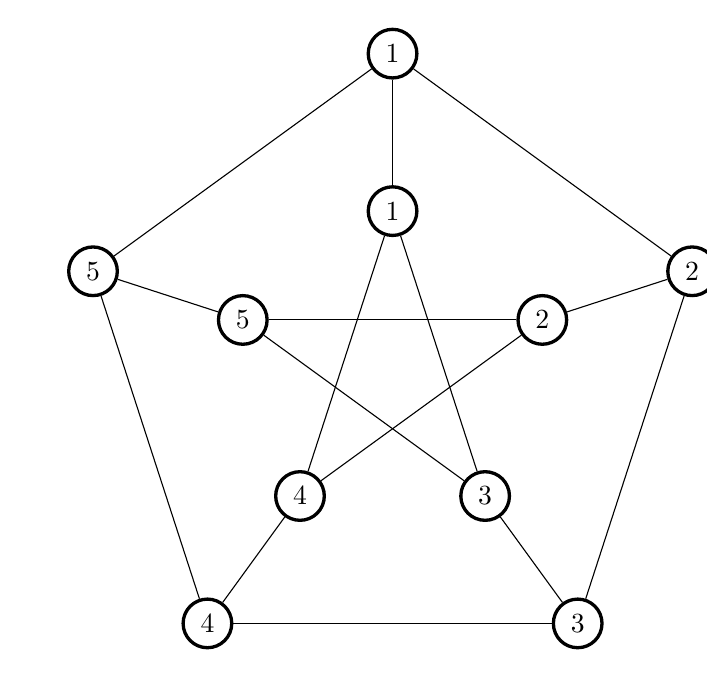
\begin{tikzpicture}[every node/.style={draw,circle,very thick}]
  \graph[clockwise, radius=4cm] {subgraph C_n [n=5,name=A] };
  \graph[clockwise, radius=2cm] {subgraph I_n [n=5,name=B] };

  \foreach \i [evaluate={\j=int(mod(\i+2+4,5)+1)}]% using Paul Gaborit's optimisation
     in {1,2,3,4,5}{
    \draw (A \i) -- (B \i);
    \draw (B \j) -- (B \i);
  }
\end{tikzpicture}
\end{figure}

\medskip

\printauthor								% Print the author data as defined above
% ------------------------------------------------------------------------------
% Begin document
% ------------------------------------------------------------------------------
\newpage
\section{Solve the following problems.}[Questions]\footnote[$\dagger$]{Dr. Yirgalem T.}

\begin{enumerate}
  \item Find $|G|,||G||,\delta(G)$ and $\Delta(G)$ for each of the following graphs
  \begin{align*}
   \text{a) }\theta_n(\text{Null graph}),\qquad \text{b) } K_n, \qquad \text{c) }P_n, \qquad \text{d) } C_n
  \end{align*}
  \item Given a graph $G$ of order $n$, and size $m$, a vertex $v\in V(G)$, and an edge $e\in E(G)$, determine the order and size of
      \begin{align*}
      \text{a) } G-v,\qquad \text{b) } G-e,\qquad \text{c) } \overline{G}
      \end{align*}
  \item Show that a regular graph of odd degree is even order.
  \item Which of the following sequences are graphic?
  \begin{align*}
   \text{a) }5,3,2,2,2 \qquad \text{b) }3,3,3,2,2 \qquad \text{c) }3,3,2,2,2 \qquad \text{d) } 3,3,3,3,2 \qquad \text{e) } 4,3,3,2,2
  \end{align*}
  \item a) Find the adjacency and incident matrix of $G=(V,E)$, where $V=\{1,2,3,4,5\}$ and
      $E=\{12,13,23,24,34,35,45\}$.\\
        b) Find the adjacency matrix for
  \begin{align*}
      \text{a) } \theta_5,\qquad \text{b) } K_5,\qquad \text{c) } C_5,\qquad \text{d) } P_5
      \end{align*}
  \item Let $G=(V,E)$, where $V=\{x,y,z,u\}$ and $E=\{xy,xz,xu,zu\}$. Draw all the subgraphs of $G$ up to isomorphism(all non isomorphic).
  \item Find two non isomorphic graph of order $5$, which are of the same degree.
  \item Which of the following graphs are isomorphic?
\begin{figure}[hbt!]
\centering
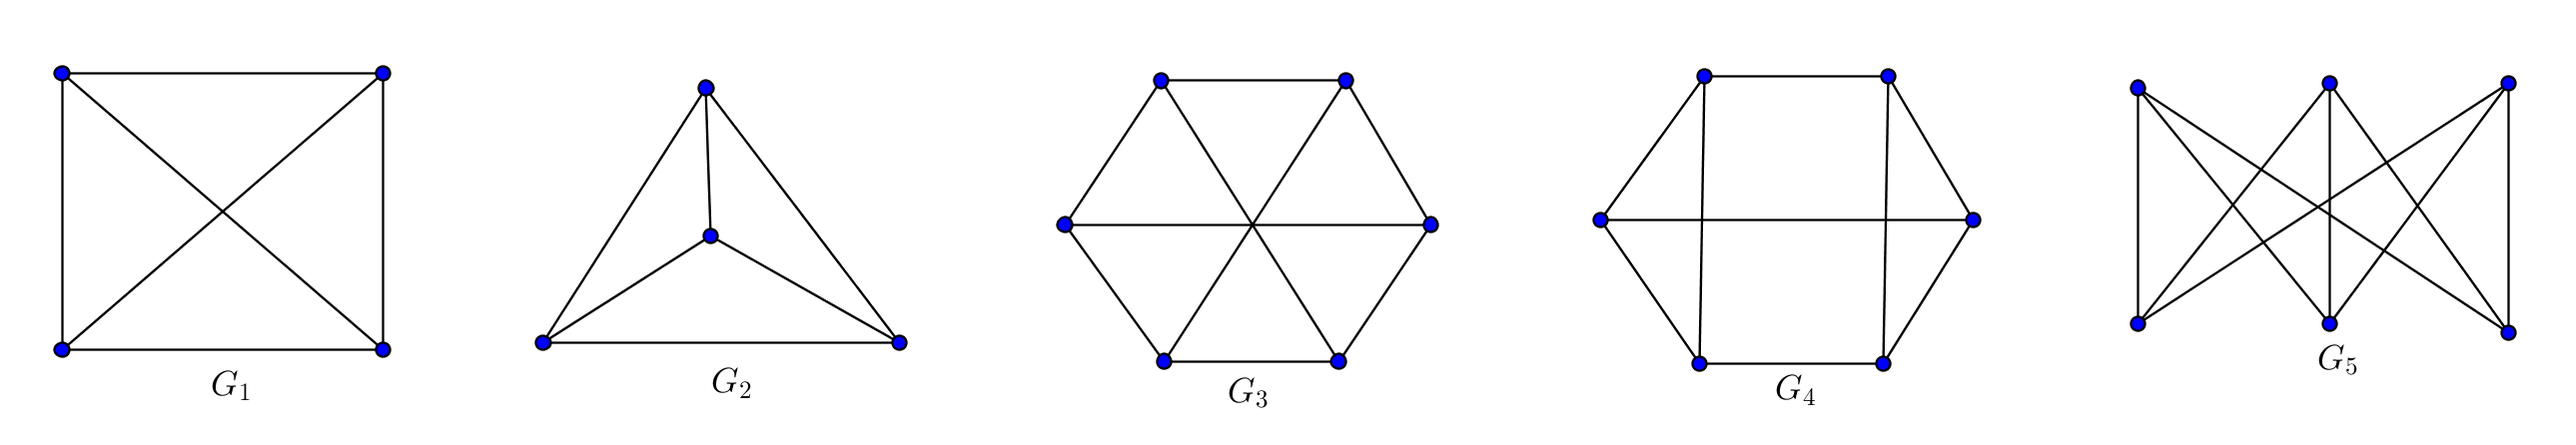
\includegraphics[width=1.0\textwidth]{GrapAss1.png}
\caption{Isomorphism}\label{fig1}
\end{figure}
\item Let $A$ be a set and $\mathfrak{B}$ be a finite collection of subsets of $A$. Then the intersection graph $I(\mathfrak{B})$ is the graph whose vertex set is $\mathfrak{B}$, and two vertices are adjacent if they are disjoint.\\
    \subitem a) Let $A=\{1,2,3,4,5,6\}$ and $\mathfrak{B}=\{\{1,2\},\{2,4\},\{1,2,3\},\{3,4,5\},\{5,6\}\}$\\
    Use diagram to show what $G=I(\mathfrak{B})$ would look like.
    \subitem b) Let $G'=(V,E)$, where $V=\{1,2,3,4\}$ and $E=\{12,23,34,41\}$. Let $S_i$ be a set consisting of the vertex $i$ and the edges incident with $i$. For instance, $S_3=\{3,23,34\}$\\
    Let
    \begin{align*}
    S=\bigcup_{i=1}^4 S_i\qquad\text{and}\qquad \mathfrak{B}=\{S_i|i=1,2,3,4\}
    \end{align*}
    Prove that $I(\mathfrak{B})\cong G'$
    \item A graph has order $13$ and $3$ components. Prove that one of its components has at least $5$ vertices.
    \item If $G$ is a simple graph of order $n$ having exactly two components which are complete graph themselves. What is the minimum and maximum possible size of $G$(in terms of $n$)?
    \item Given the graphs you see below, determine the smallest number of vertices that have to be removed from $G$ to disconnect $G$(which vertices)?
  \begin{figure}[hbt!]
\centering
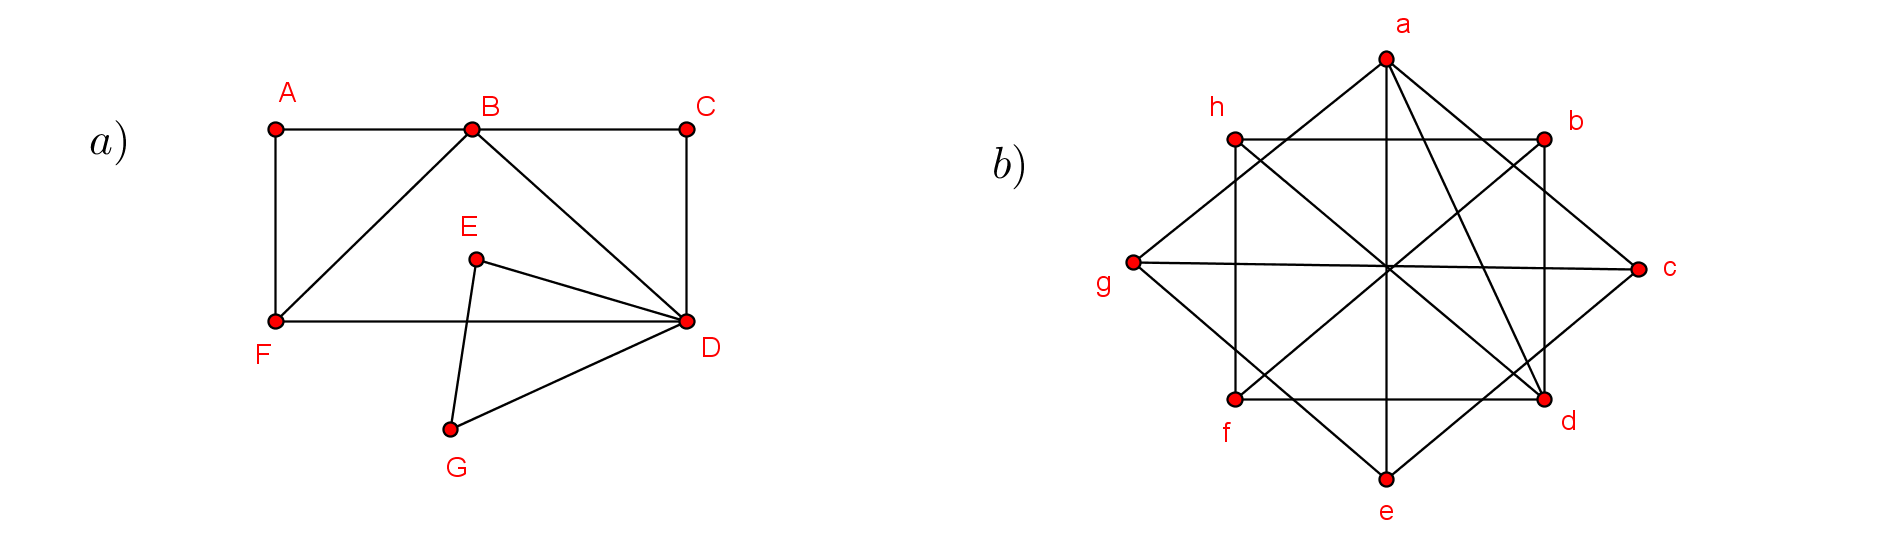
\includegraphics[width=1.0\textwidth]{GrapAss2.png}
\caption{Disconnect}\label{fig2}
\end{figure}
  \item Let $G=(V,E)$, where $V=\{1,2,\ldots,15\}$, and two vertices $i$ and $j$ are adjacent iff greatest common divisor $\gcd(i,j)\neq 1$.
  \begin{align*}
      \text{a) Draw $G$} ,\qquad \text{b) How long is the longest path in $G$?}
      \end{align*}
  \item Find the diameters of
  \begin{align*}
      \text{a) The peterson graph,} \quad \text{b) The hypercube $Q_n$},\quad \text{c) } K_n\qquad \text{d) } K_{n,m} \qquad \text{e) } C_n \qquad \text{f) } P_n
  \end{align*}
  \item Which of the following graphs are \\
  a) Eulerian $\qquad$ b) Hamiltonian
  \begin{figure}[hbt!]
\centering
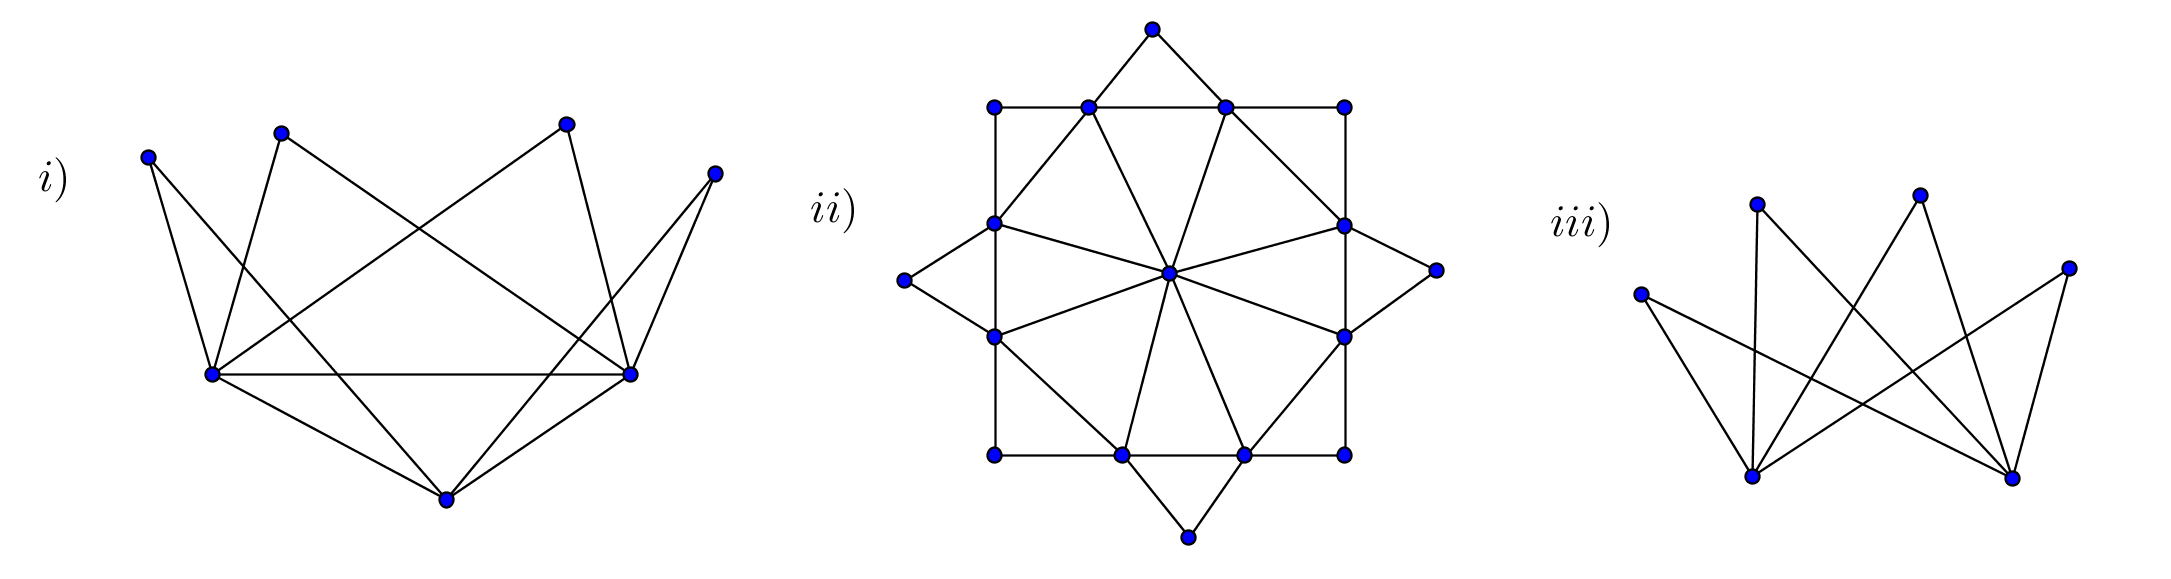
\includegraphics[width=1.0\textwidth]{GrapAss3.png}
\caption{Eulerian and Hamiltonian}\label{fig3}
\end{figure}
  \item Show that if a graph is regular and of even order and odd size, then it is not Eulerian\footnote{Leonhard Euler (1707-1783) a prolific Swiss mathematician. In 1735, Euler presented a solution to the problem known as the {\color{blue} Seven Bridges of K\"{o}nigsberge}, which made him the father of graph theory.}.
  \newpage
  \item Which of the following diagram could be drawn without lifting your pen from the paper and without repeating any line?
\begin{figure}[hbt!]
\centering
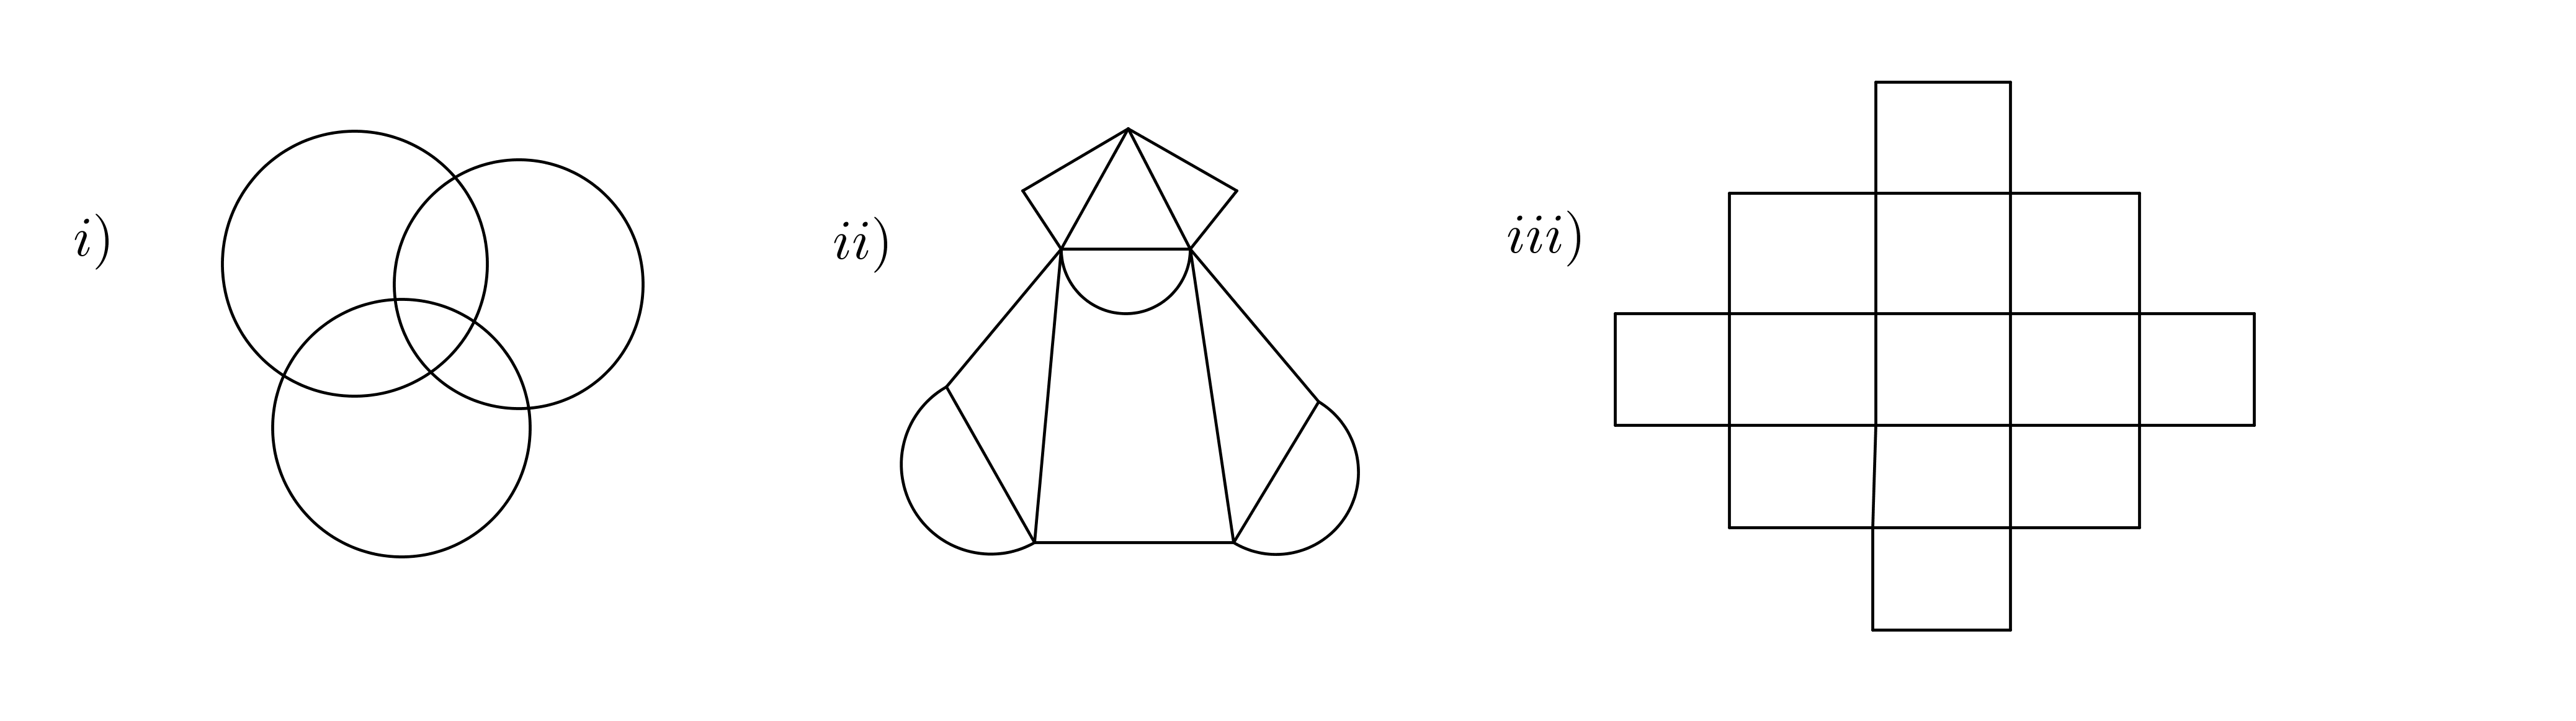
\includegraphics[width=1.0\textwidth]{GrapAss4.png}
\caption{Euler trail}\label{fig4}
\end{figure}
  \item Take $n=6$, and let $m\le \frac{n}{2}, m\in \mathbb{N}$.
  \begin{description}
    \item[a)] Draw the graph $K_m\vee\footnote{Join operator "$\vee$"} (\overline{K_m}+\footnote{Disjoint Union operator "+"} K_{n-2m})$, (for each $m\le \frac{n}{2}$).
    \item[b)] Show that this graphs can not be Hamiltonian.
    \item[c)] Give the degree sequence of each of the graphs you obtained in (a) above, in a decreasing order.
    \item[d)] Is it possible to find a non-Hamiltonian graph of the same order which degree majorizes any of these graphs? why?
  \end{description}
  \item What is the minimum number of edges a simple graph $G$ of order $n\geq2$ should have to guarantee that it is Hamiltonian.
  \item Find the degree sequence of the non-Hamiltonian simple graph with $n$ vertices and $\binom{n-1}{2}+1$ edges.
  \item Let $T$ be a tree of order $12$ that has exactly $3$ vertices of degree $3$ and one of degree $2$. Give the degree sequence of $T$.
  \item Show that the sequence $7,2,2,1,1,1,1,1,1,1$ is a degree sequence of a tree.
  \item Compute the number of spanning tree of $K_{10}$.
  \item a) Find the Pr\"{u}fer sequence corresponding to the tree of order $11$ with $V=\{1,2,\ldots,11\}$ and $E=\{12,13,24,25,36,37,48,49,510,511\}$.\\
        b) Construct a tree that have the Pr\"{u}fer code $4,5,7,2,1,1,6,6,7$.
  \item Let $G$ be a forest\footnote{A forest is simply an acyclic graph(A disconnected graph whose components are tree).} having $m$ components. How many edges should be added to $G$ to obtain a tree containing $G$?
  \item a) What is the minimum number of leaves a tree can have if the order $n\ge2$?(Express your answer in terms of some basic element of a graph)\\
      b) What is the maximum number of leaves in a tree of order $n$?
  \newpage
  \item Find a matching , a maximum matching or a perfect matching or explain why it does not exist in the following graph.
  \begin{figure}[hbt!]
\centering
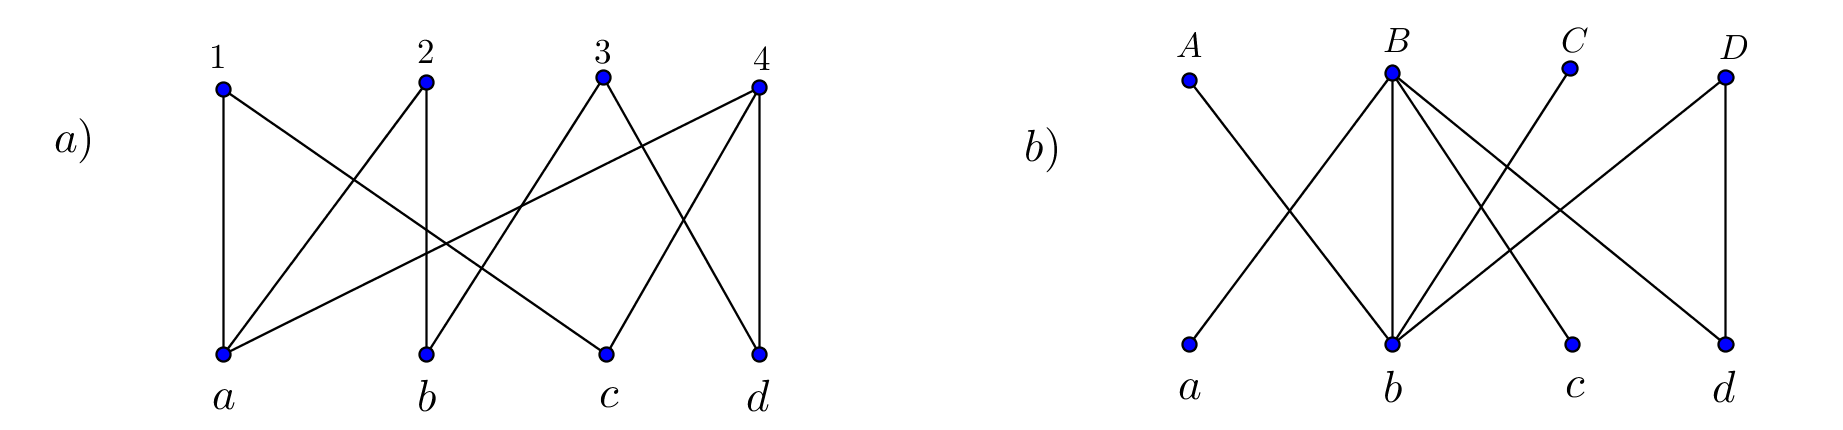
\includegraphics[width=1.0\textwidth]{GrapAss5.png}
\caption{Matching}\label{fig5}
\end{figure}
  \item Is there a job for each of the applicant in $\{A,B,C,D,E\}$ if the jobs are $a,b,c,d$ and $e$(in $G$ below)?
    \begin{figure}[hbt!]
\centering
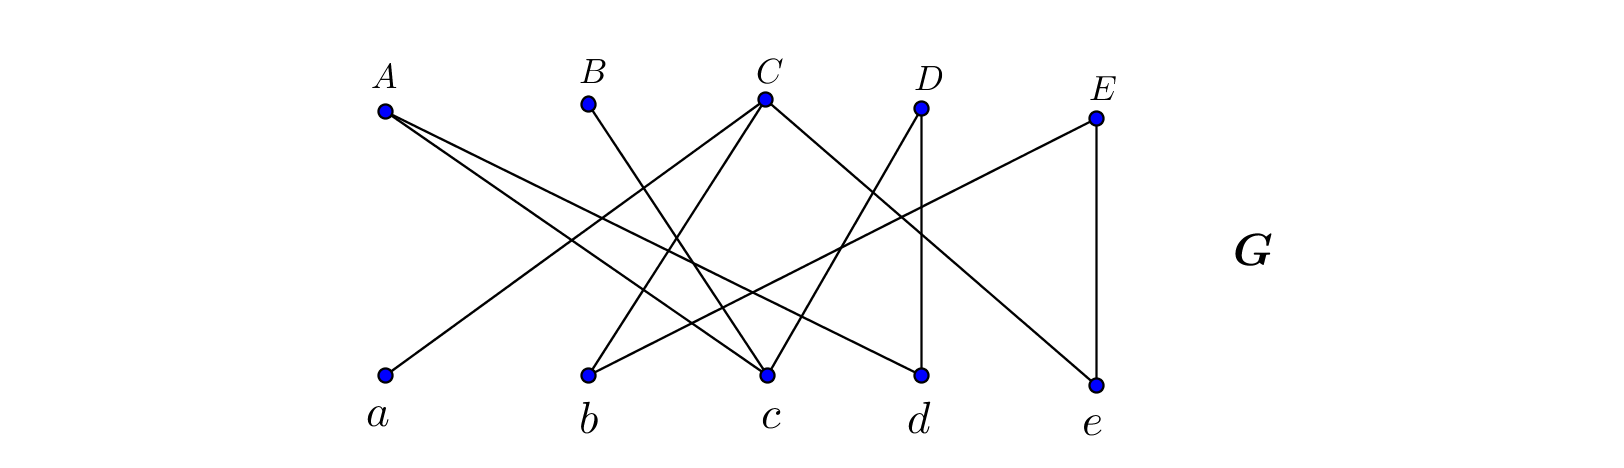
\includegraphics[width=1.0\textwidth]{GrapAss6.png}
\caption{Applicant-Job}\label{fig6}
\end{figure}
  \item A connected plane graph of order $n$ is $4$-regular and has $10$ faces(regions). What is the value of $n$?
  \item For which values of $n$ is $K_n$ planar?
  \item For which values of $n$ and $m$ is $K_{n,m}$ planar?
  \item For a graph $G$ below
  \begin{figure}[hbt!]
\centering
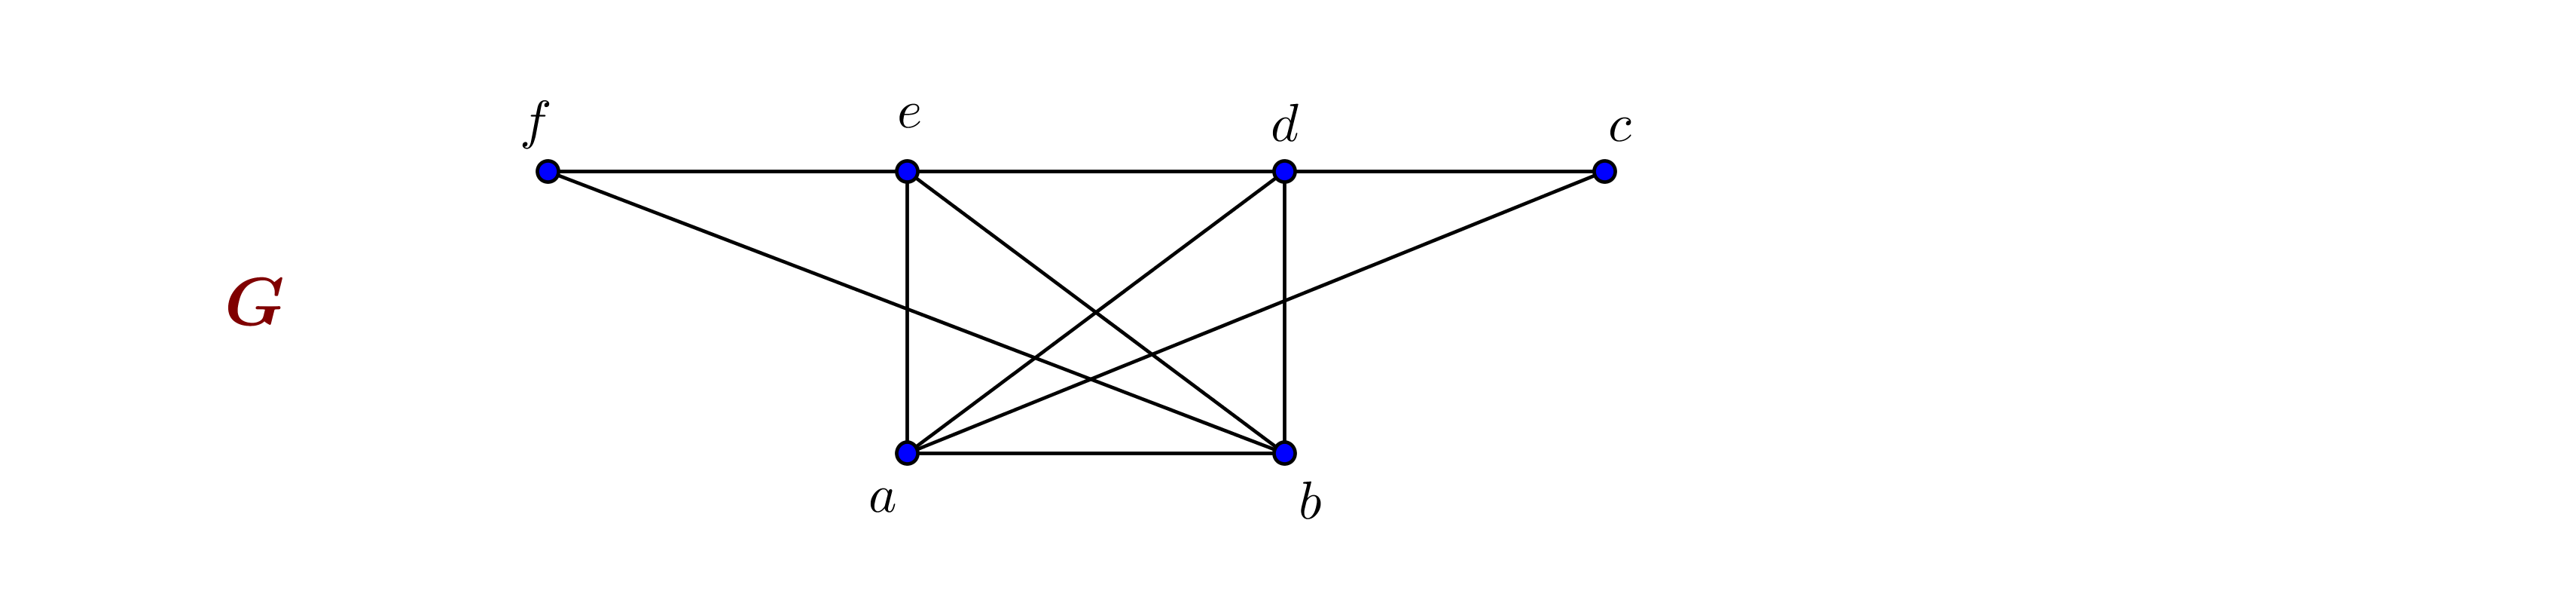
\includegraphics[width=1.0\textwidth]{GrapAss7.png}
\caption{Dual}\label{fig7}
\end{figure}

Draw the dual of $G$ and show that
  \begin{align*}
  \sum_{\text{all faces}}\deg(\text{faces})=2|E|
  \end{align*}
\end{enumerate}
\section{Solutions}[Answers]\footnote[$\ddag$]{Miliyon T.}
\begin{enumerate}
  \item For $\#1$ look the table below

  \begin{table}[!htb]
\centering
\begin{tabular}{ l | c|c|c|c| r | }
                 & $a$         & $b$                & $c$   & $d$   \\ \hline
    $G$          & $\theta_n$  & $K_n$              & $P_n$ & $C_n$ \\ \hline
    $|G|$        & $n$         & $n$                & $n$   & $n$  \\ \hline
    $\|G\|$      & $0$         & $\frac{n(n-1)}{2}$ & $n-1$ & $n$  \\ \hline
    $\delta(G)$  & $0$         & $n-1$              & $1$   & $2$  \\ \hline
    $\Delta(G)$  & $0$         & $n-1$              & $2$   & $2$  \\
    \hline
  \end{tabular}
  \caption{Question 1}
\end{table}
  \item Given that $|G|=n$ and $\|G\|=m$

  \begin{table}[!htb]
\centering
\begin{tabular}{ l|c|c|c|r |}
               & $a$         & $b$     &  $c$ \\ \hline
    $G$        & $G-v$       & $G-e$   & $\overline{G}$   \\ \hline
    $|G|$      & $n-1$       & $n$     & $n$ \\ \hline
    $\|G\|$    & $m-\deg(v)$ & $m-1$   & $\|K_n\|-\|G\|=\frac{n(n-1)}{2}-m$   \\
    \hline
  \end{tabular}
  \caption{Question 2}
\end{table}

  \item Let $G$ be a regular graph of odd degree. Denote that odd degree by $d$(odd). We wand to show $|G|$ is even.\\
      Suppose not(i.e. $|G|$ is odd). For simplicity denote $|G|=k$(odd).\\
      As $G$ is regular every $v\in V(G)$ is of degree $d$(which is odd) and we have $k$ vertices. Thus
      \begin{align*}
      \sum_{v\in V(G)}\deg(v)=\underbrace{d}_{odd}\cdot\underbrace{k}_{odd}=\text{ odd number}
      \end{align*}
  Notice that both $d$ and $k$ are odd, then their product(which is by definition the sum of degrees in $G$) must be odd. But from Handshaking lemma we know that such thing(the sum of degree in any graph being odd) will never happen(ever!). Hence a contradiction! our assumption was incorrect.\\
  $\therefore\ |G|$ is even.

  \item The necessary and sufficient condition for any sequence of numbers to be \textbf{graphic} given by the following fact.
  \begin{thm}\footnote{This result is due to Hungarian mathematicians Erd\H{o}s and Gallai}
  A non-increasing sequence of non-negative integers $d_1,d_2,\ldots,d_n$ is \textbf{graphical} iff its sum is even and for $k=1,2,\ldots,n$
  \begin{align}\label{erdosgali}
  \sum_{i=1}^{k}d_i\leq k(k-1)+\sum_{i=k+1}^{n}\min\{d_i,n\}
  \end{align}
  \end{thm}
  We use (\ref{erdosgali}) to show the sequence in (a) is not \textbf{graphic}\\
  \newpage
  (a) $5,3,2,2,2$ $n=5$.\\
  For $k=1$
  \begin{align*}
  \sum_{i=1}^{1}d_i=5&\leq 1(1-1)+\sum_{i=2}^{5}\min\{d_i,1\}\\
                     &\leq 0+(1+1+1+1)\\
                     &\leq 4\\
  \Rightarrow 5 &\leq 4 \qquad \rightarrow\leftarrow
  \end{align*}
  Hence the sequence given above is not \textbf{graphic}.\\
  (b) $3,3,3,2,2$\\
  This sequence is not \textbf{graphic} since its sum is not even on the first place.
  \medskip

  Thanks to Havel and Hakimi, we are able to construct the corresponding simple graphs for the sequences given in (c),(d) and (e)\\
  (c) $3,3,2,2,2$
\begin{figure}[hbt!]
\centering
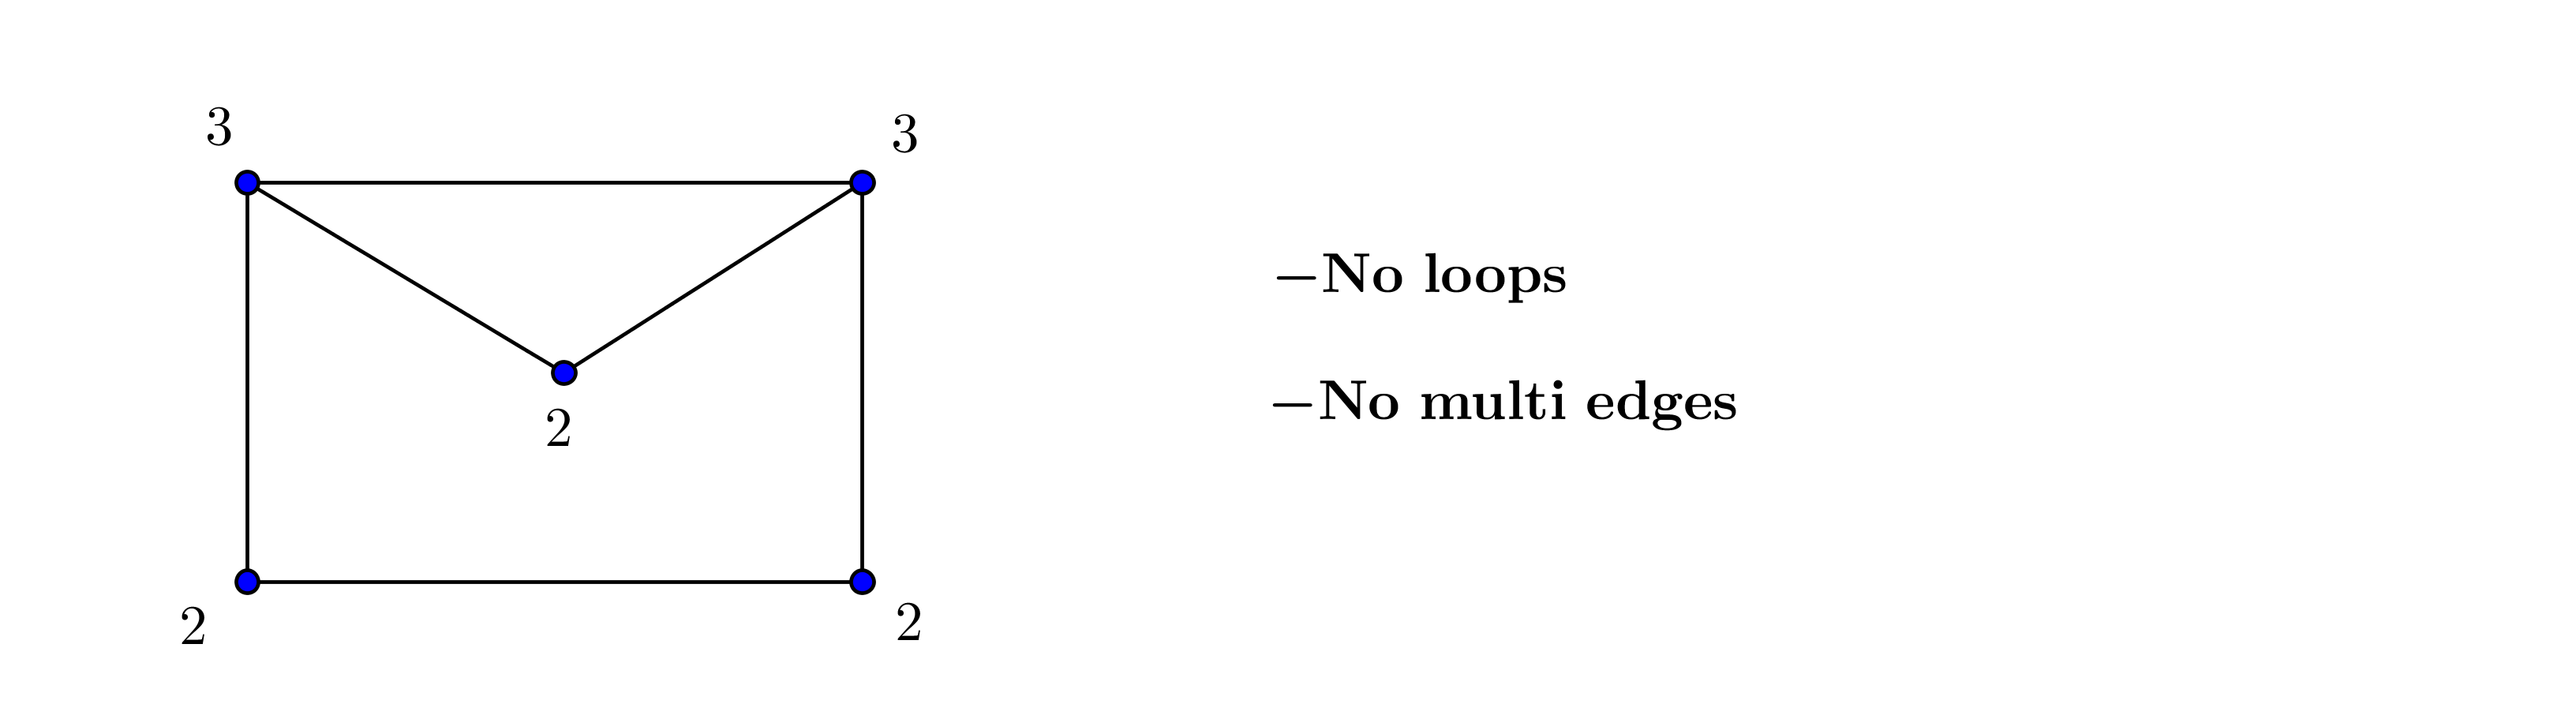
\includegraphics[width=.9\textwidth]{SolGrapAssc.png}
\end{figure}

  (d) $3,3,3,3,2$

  \begin{figure}[hbt!]
\centering
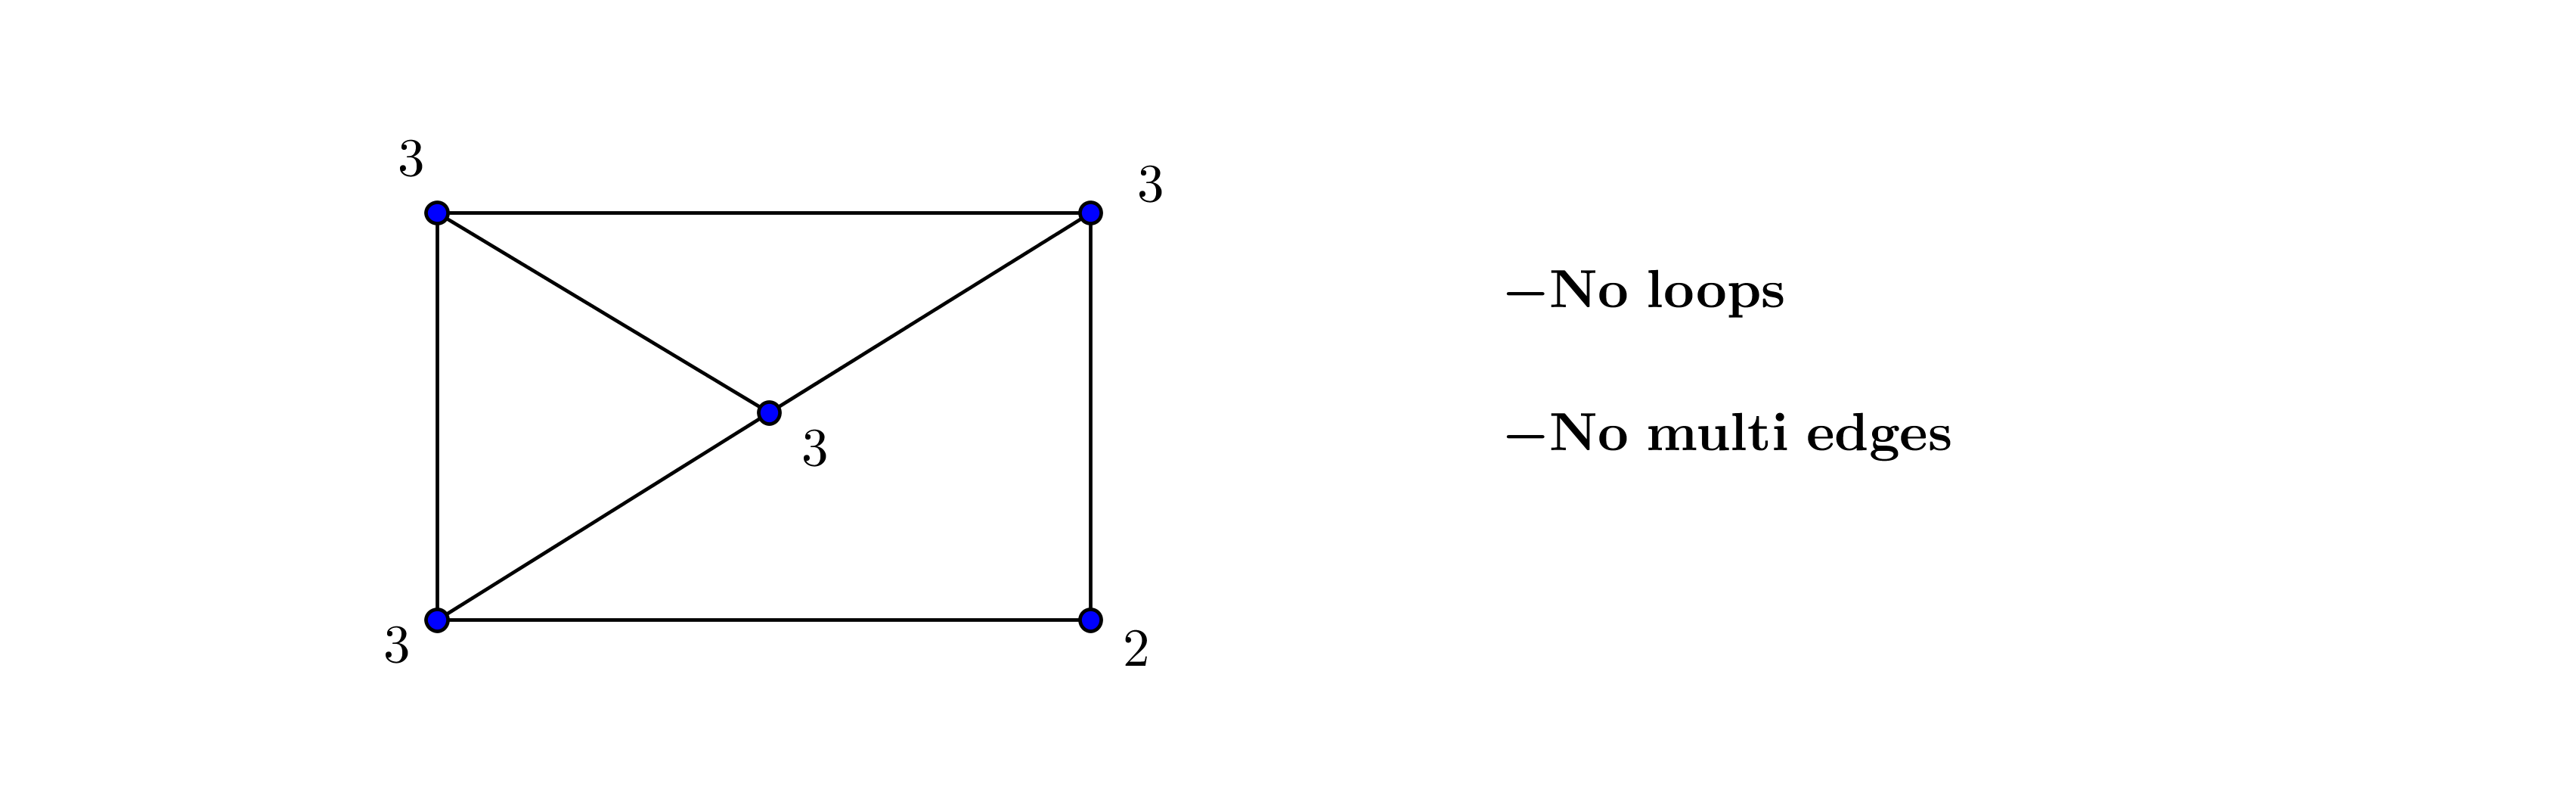
\includegraphics[width=.9\textwidth]{SolGrapAssd.png}
\end{figure}

  (e) $4,3,3,2,2$

  \begin{figure}[hbt!]
\centering
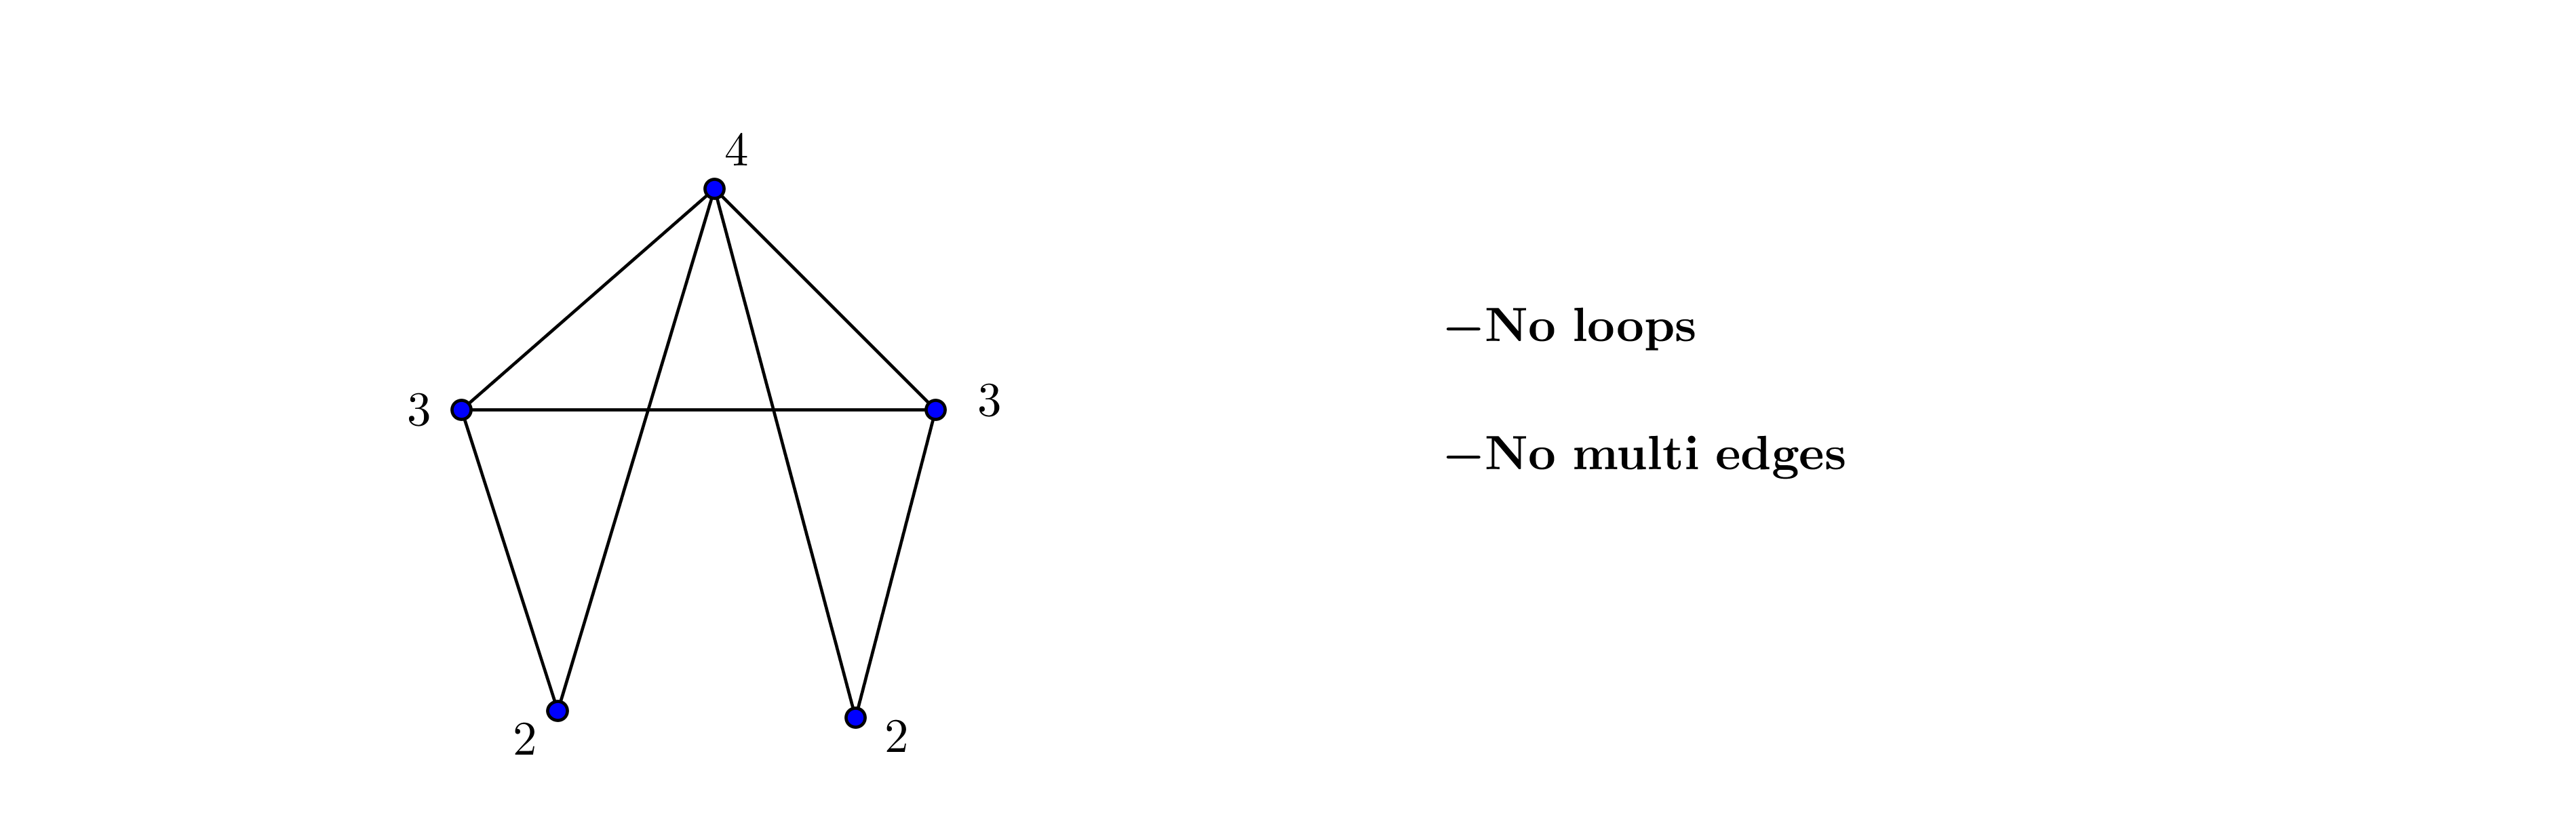
\includegraphics[width=.9\textwidth]{SolGrapAsse.png}
\end{figure}

\newpage

  \item (a) For graph $G$ below

 \begin{figure}[hbt!]
\centering
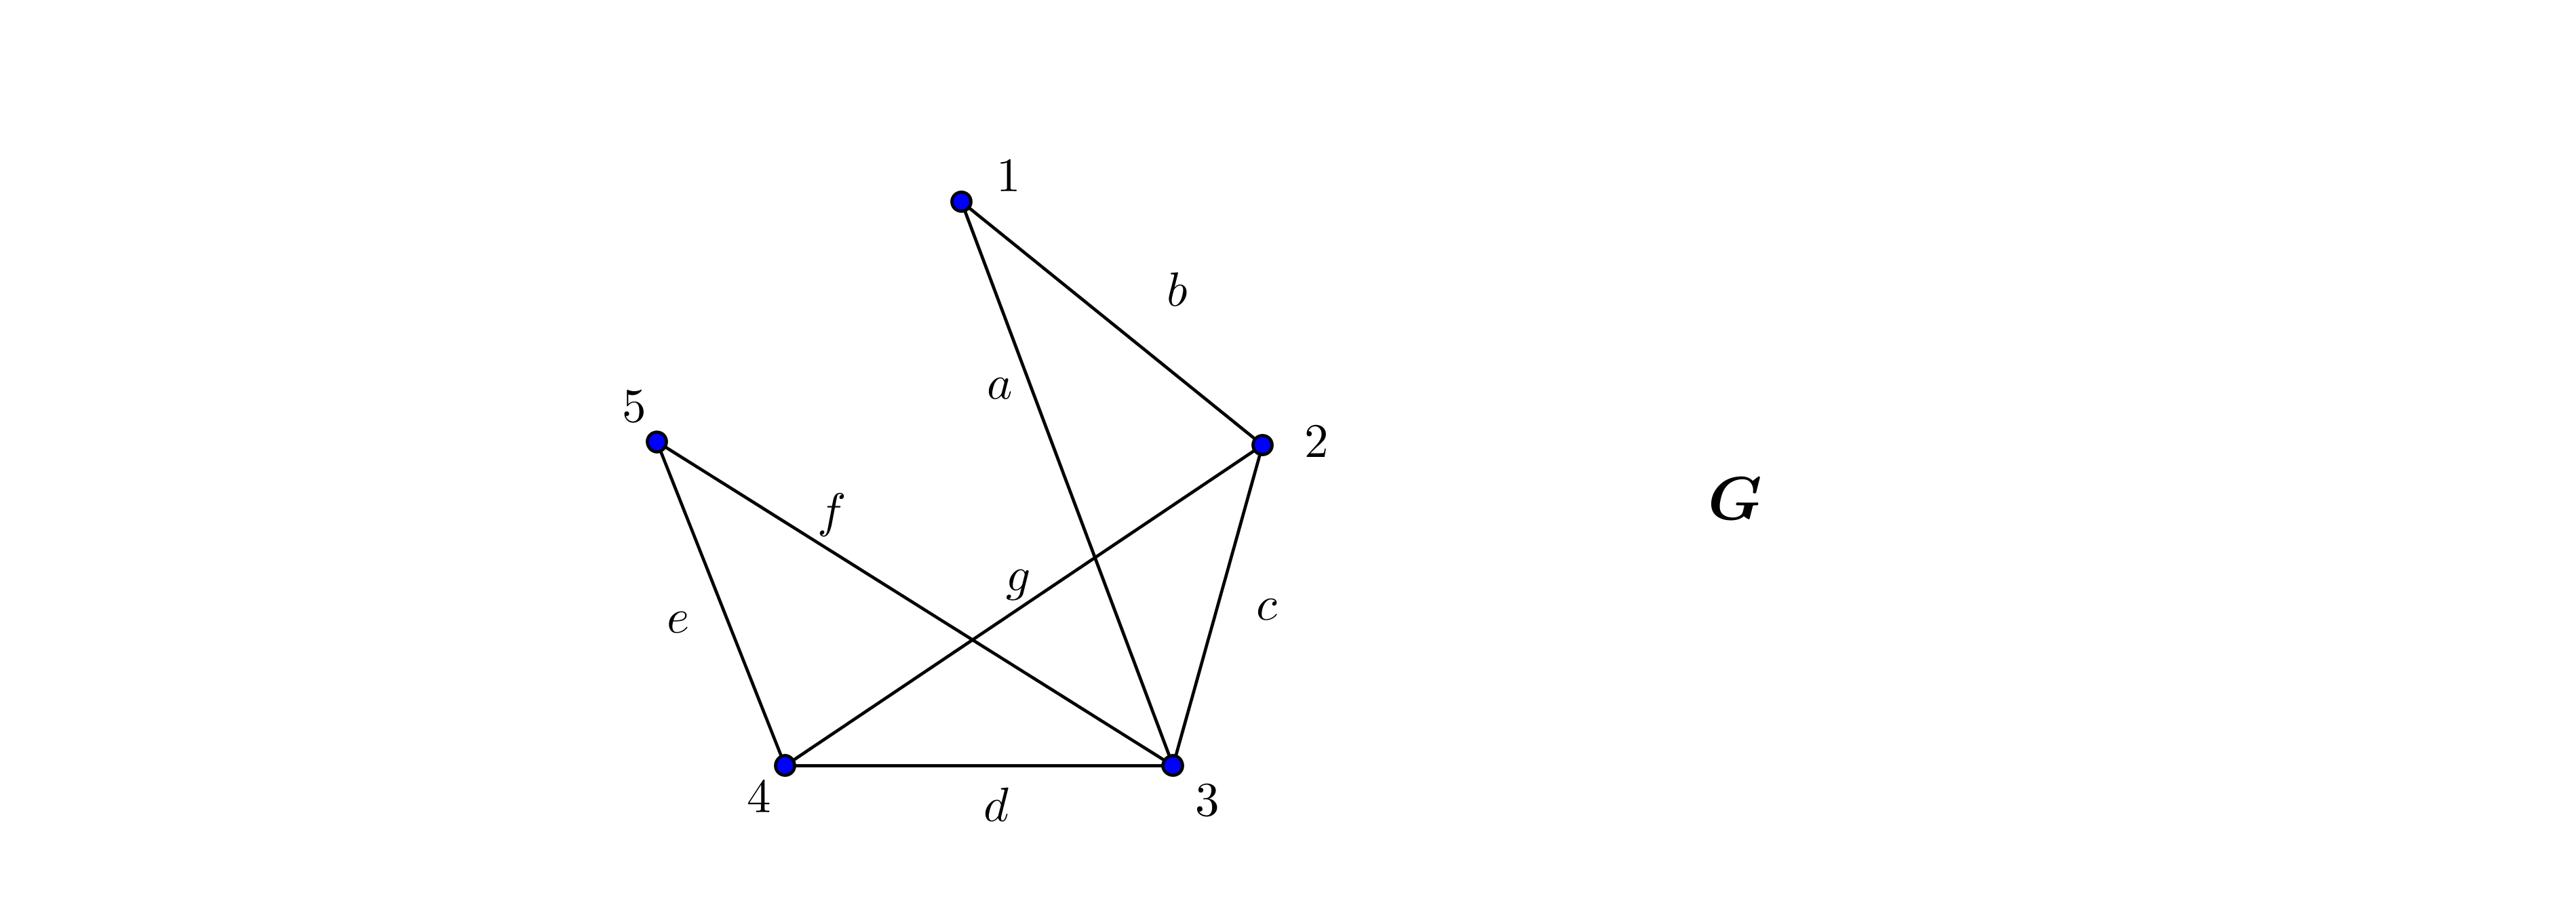
\includegraphics[width=.9\textwidth]{SolGrapAss5a.png}
\end{figure}
The adjacency matrix of $G$ is

\[
\begin{array}{c|cccccccccccccccccc}
         & 1 & 2 & 3 & 4 & 5 \\ \hline
     1 & 0 & 1 & 1 & 0 & 0 \\
     2 & 1 & 0 & 1 & 1 & 0 \\
     3 & 1 & 1 & 0 & 1 & 1 \\
     4 & 0 & 1 & 1 & 0 & 1 \\
     5 & 0 & 0 & 1 & 1 & 0
\end{array} \qquad \Rightarrow\qquad
A_G=\left(
    \begin{matrix}
      0 & 1 & 1 & 0 & 0 \\
      1 & 0 & 1 & 1 & 0 \\
      1 & 1 & 0 & 1 & 1 \\
      0 & 1 & 1 & 0 & 1 \\
      0 & 0 & 1 & 1 & 0
    \end{matrix}
    \right)
\]

The incident matrix of $G$ is

\[
\begin{array}{c|cccccccccccccccccc}
       & a & b & c & d & e & f & g \\ \hline
     1 & 1 & 1 & 0 & 0 & 0 & 0 & 0 \\
     2 & 0 & 1 & 1 & 0 & 0 & 0 & 1\\
     3 & 1 & 0 & 1 & 1 & 0 & 1 & 0\\
     4 & 0 & 0 & 0 & 1 & 1 & 0 & 1\\
     5 & 0 & 0 & 0 & 0 & 1 & 1 & 0
\end{array} \qquad \Rightarrow\qquad
M_G=\begin{bmatrix}
      1 & 1 & 0 & 0 & 0 & 0 & 0 \\
      0 & 1 & 1 & 0 & 0 & 0 & 1\\
      1 & 0 & 1 & 1 & 0 & 1 & 0\\
      0 & 0 & 0 & 1 & 1 & 0 & 1\\
      0 & 0 & 0 & 0 & 1 & 1 & 0
    \end{bmatrix}
\]
(b)
\begin{description}
  \item[i)] The adjacency matrix for $\theta_5$ is

$$
 (0)_{5\times5},\qquad \text{null matrix of order 5.}
$$

  \item[ii)] The adjacency matrix for $K_5$
$$
\left(
    \begin{matrix}
      0 & 1 & 1 & 1 & 1 \\
      1 & 0 & 1 & 1 & 1 \\
      1 & 1 & 0 & 1 & 1 \\
      1 & 1 & 1 & 0 & 1 \\
      1 & 1 & 1 & 1 & 0
    \end{matrix}
    \right)
$$

  \item[iii)] The adjacency matrix for $P_5$
$$
\left(
    \begin{matrix}
      0 & 1 & 0 & 0 & 0 \\
      1 & 0 & 1 & 0 & 0 \\
      0 & 1 & 0 & 1 & 0 \\
      0 & 0 & 1 & 0 & 1 \\
      0 & 0 & 0 & 1 & 0
    \end{matrix}
    \right)
$$

  \item[iv)] The adjacency matrix for $C_5$
$$
\left(
    \begin{matrix}
      0 & 1 & 0 & 0 & 1 \\
      1 & 0 & 1 & 0 & 0 \\
      0 & 1 & 0 & 1 & 0 \\
      0 & 0 & 1 & 0 & 1 \\
      1 & 0 & 0 & 1 & 0
    \end{matrix}
    \right)
$$
\end{description}
  \item  Let $G=(V,E)$, where $V=\{x,y,z,u\}$ and $E=\{xy,xz,xu,zu\}$. Which can be drawn

  \begin{figure}[hbt!]
\centering
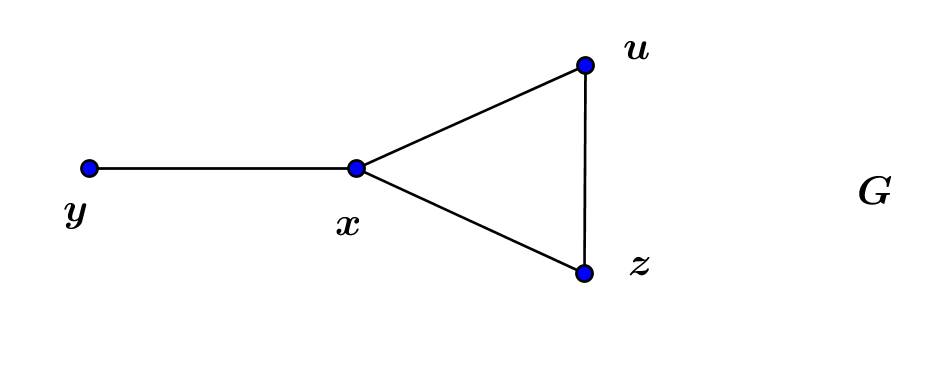
\includegraphics[width=.5\textwidth]{SolGrapAsub.png}
\end{figure}
The non isomorphic subgraphs of $G$ are
\begin{figure}[hbt!]
\centering
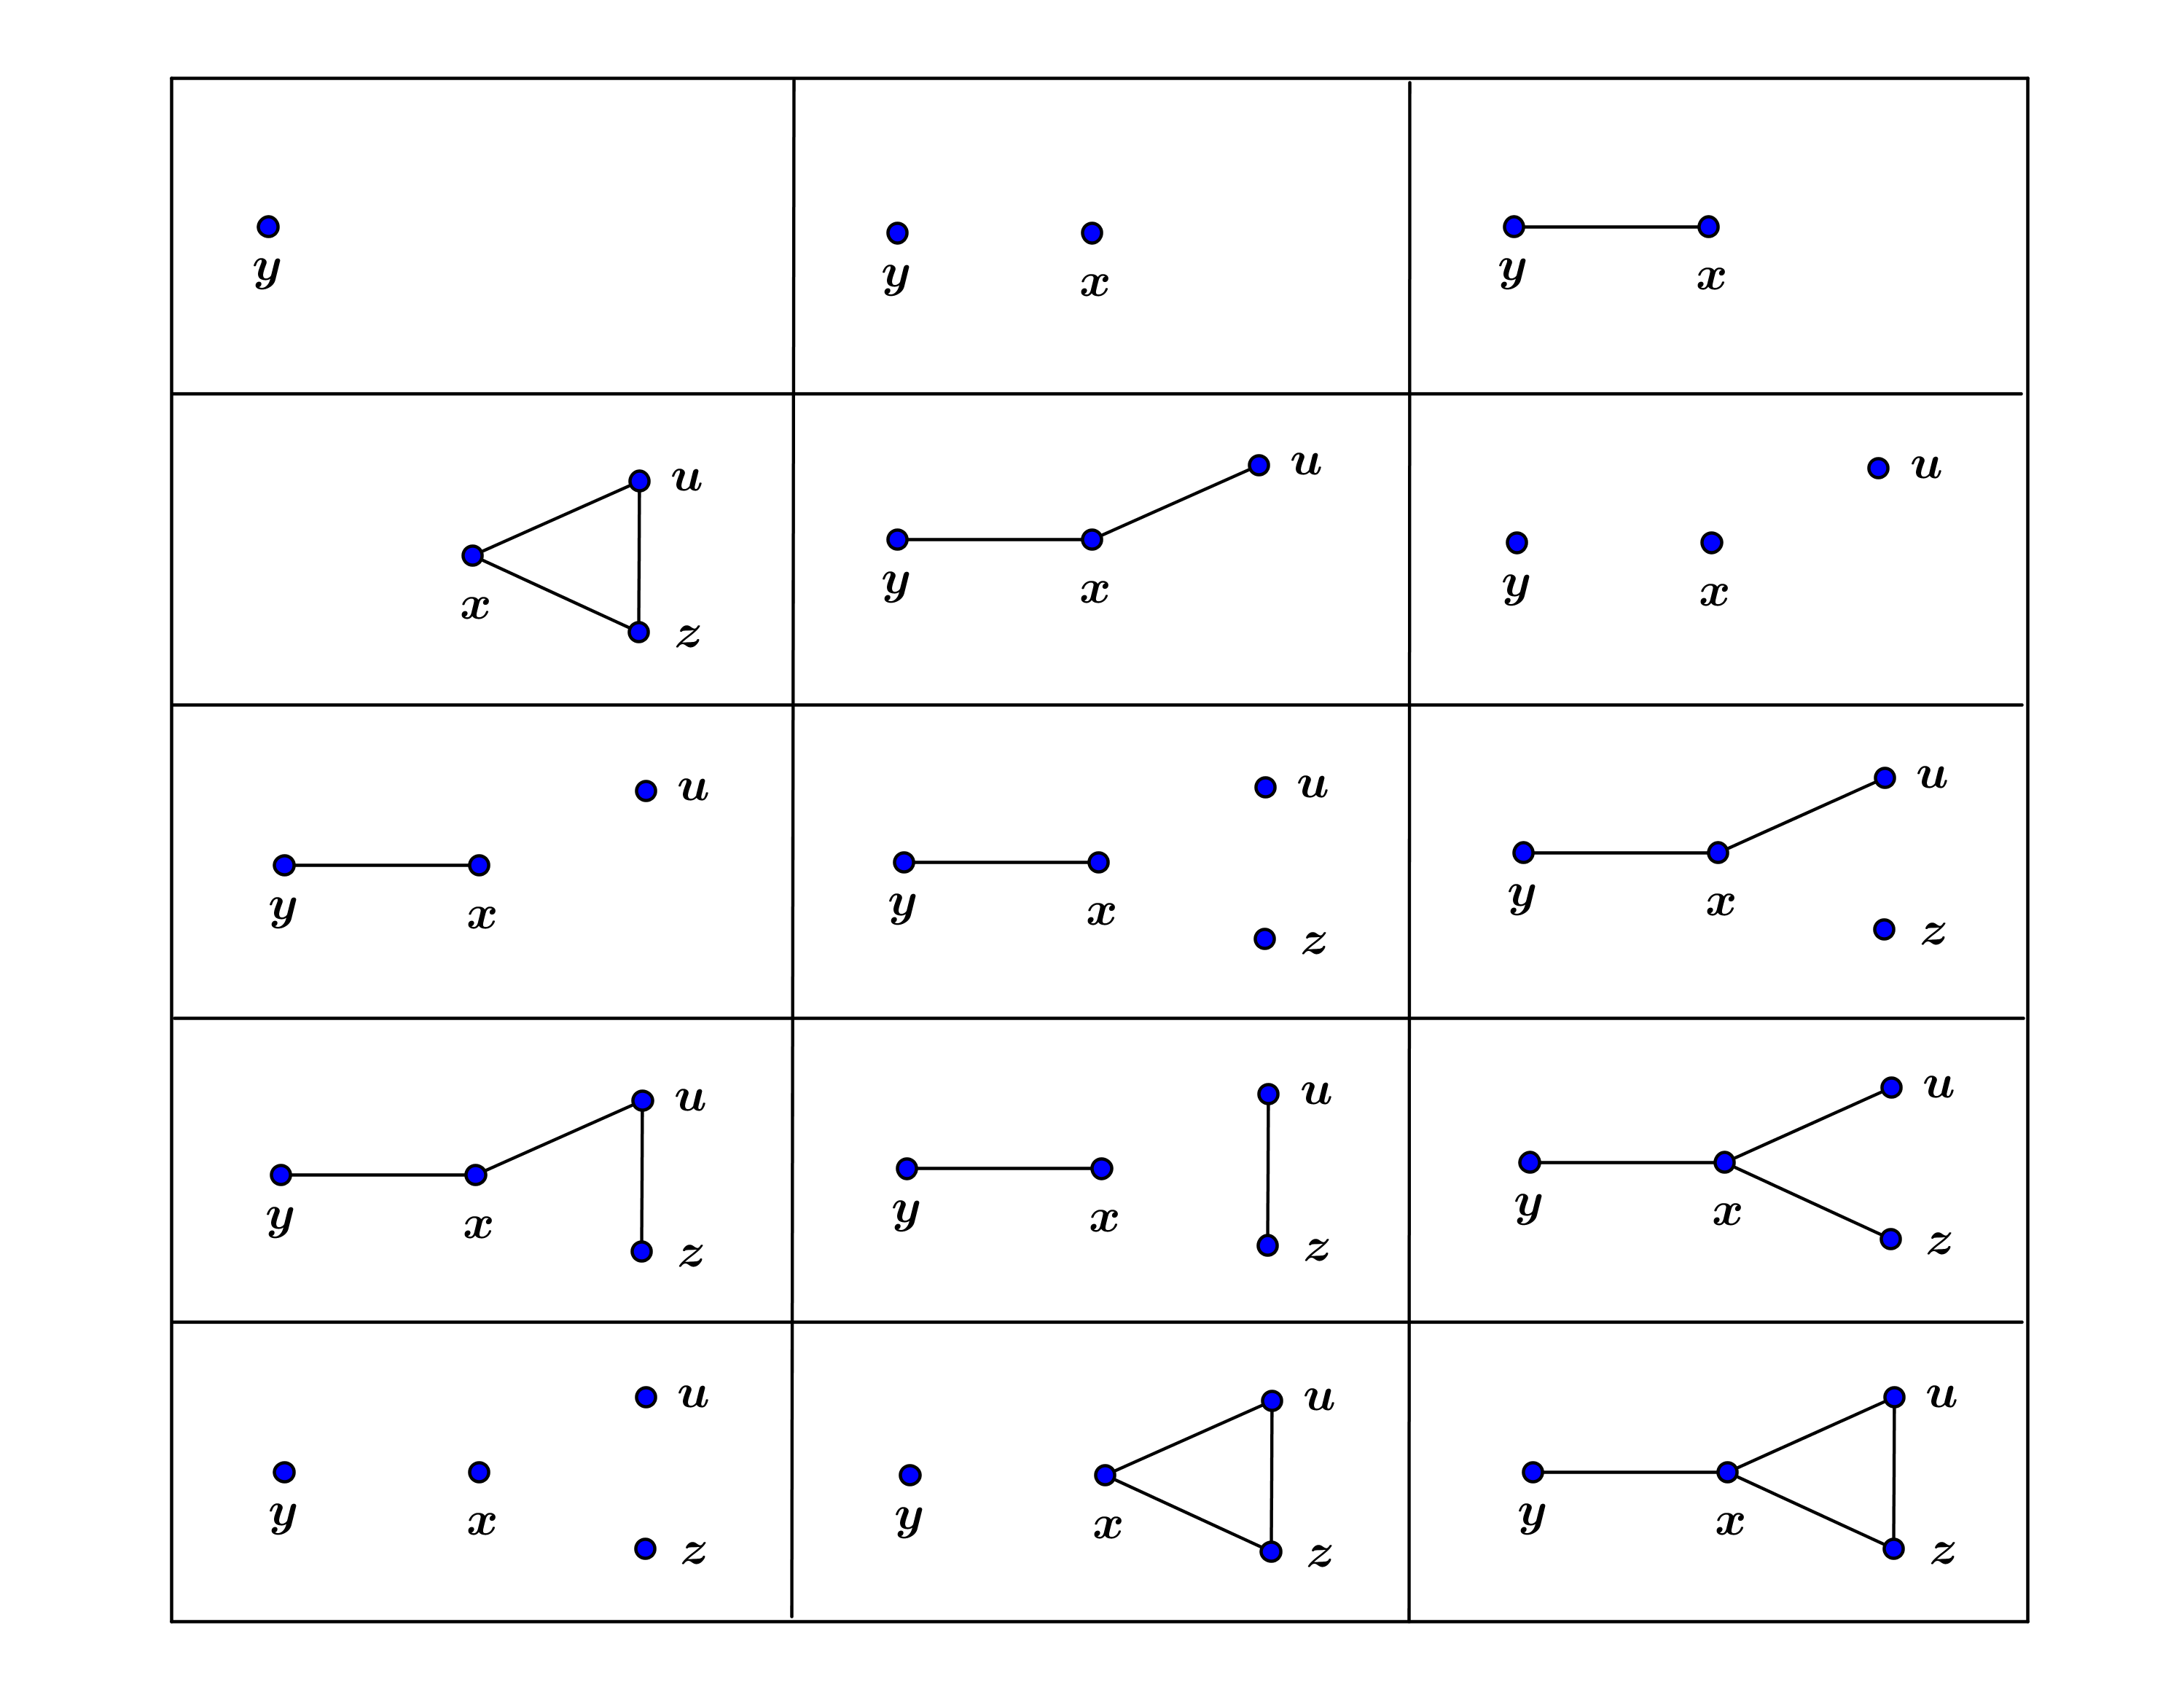
\includegraphics[width=1.03\textwidth]{SolGrapAsubgraph.png}
\end{figure}

  \newpage
  \item $G_1$ and $G_2$ below are one such example.
  \begin{figure}[hbt!]
\centering
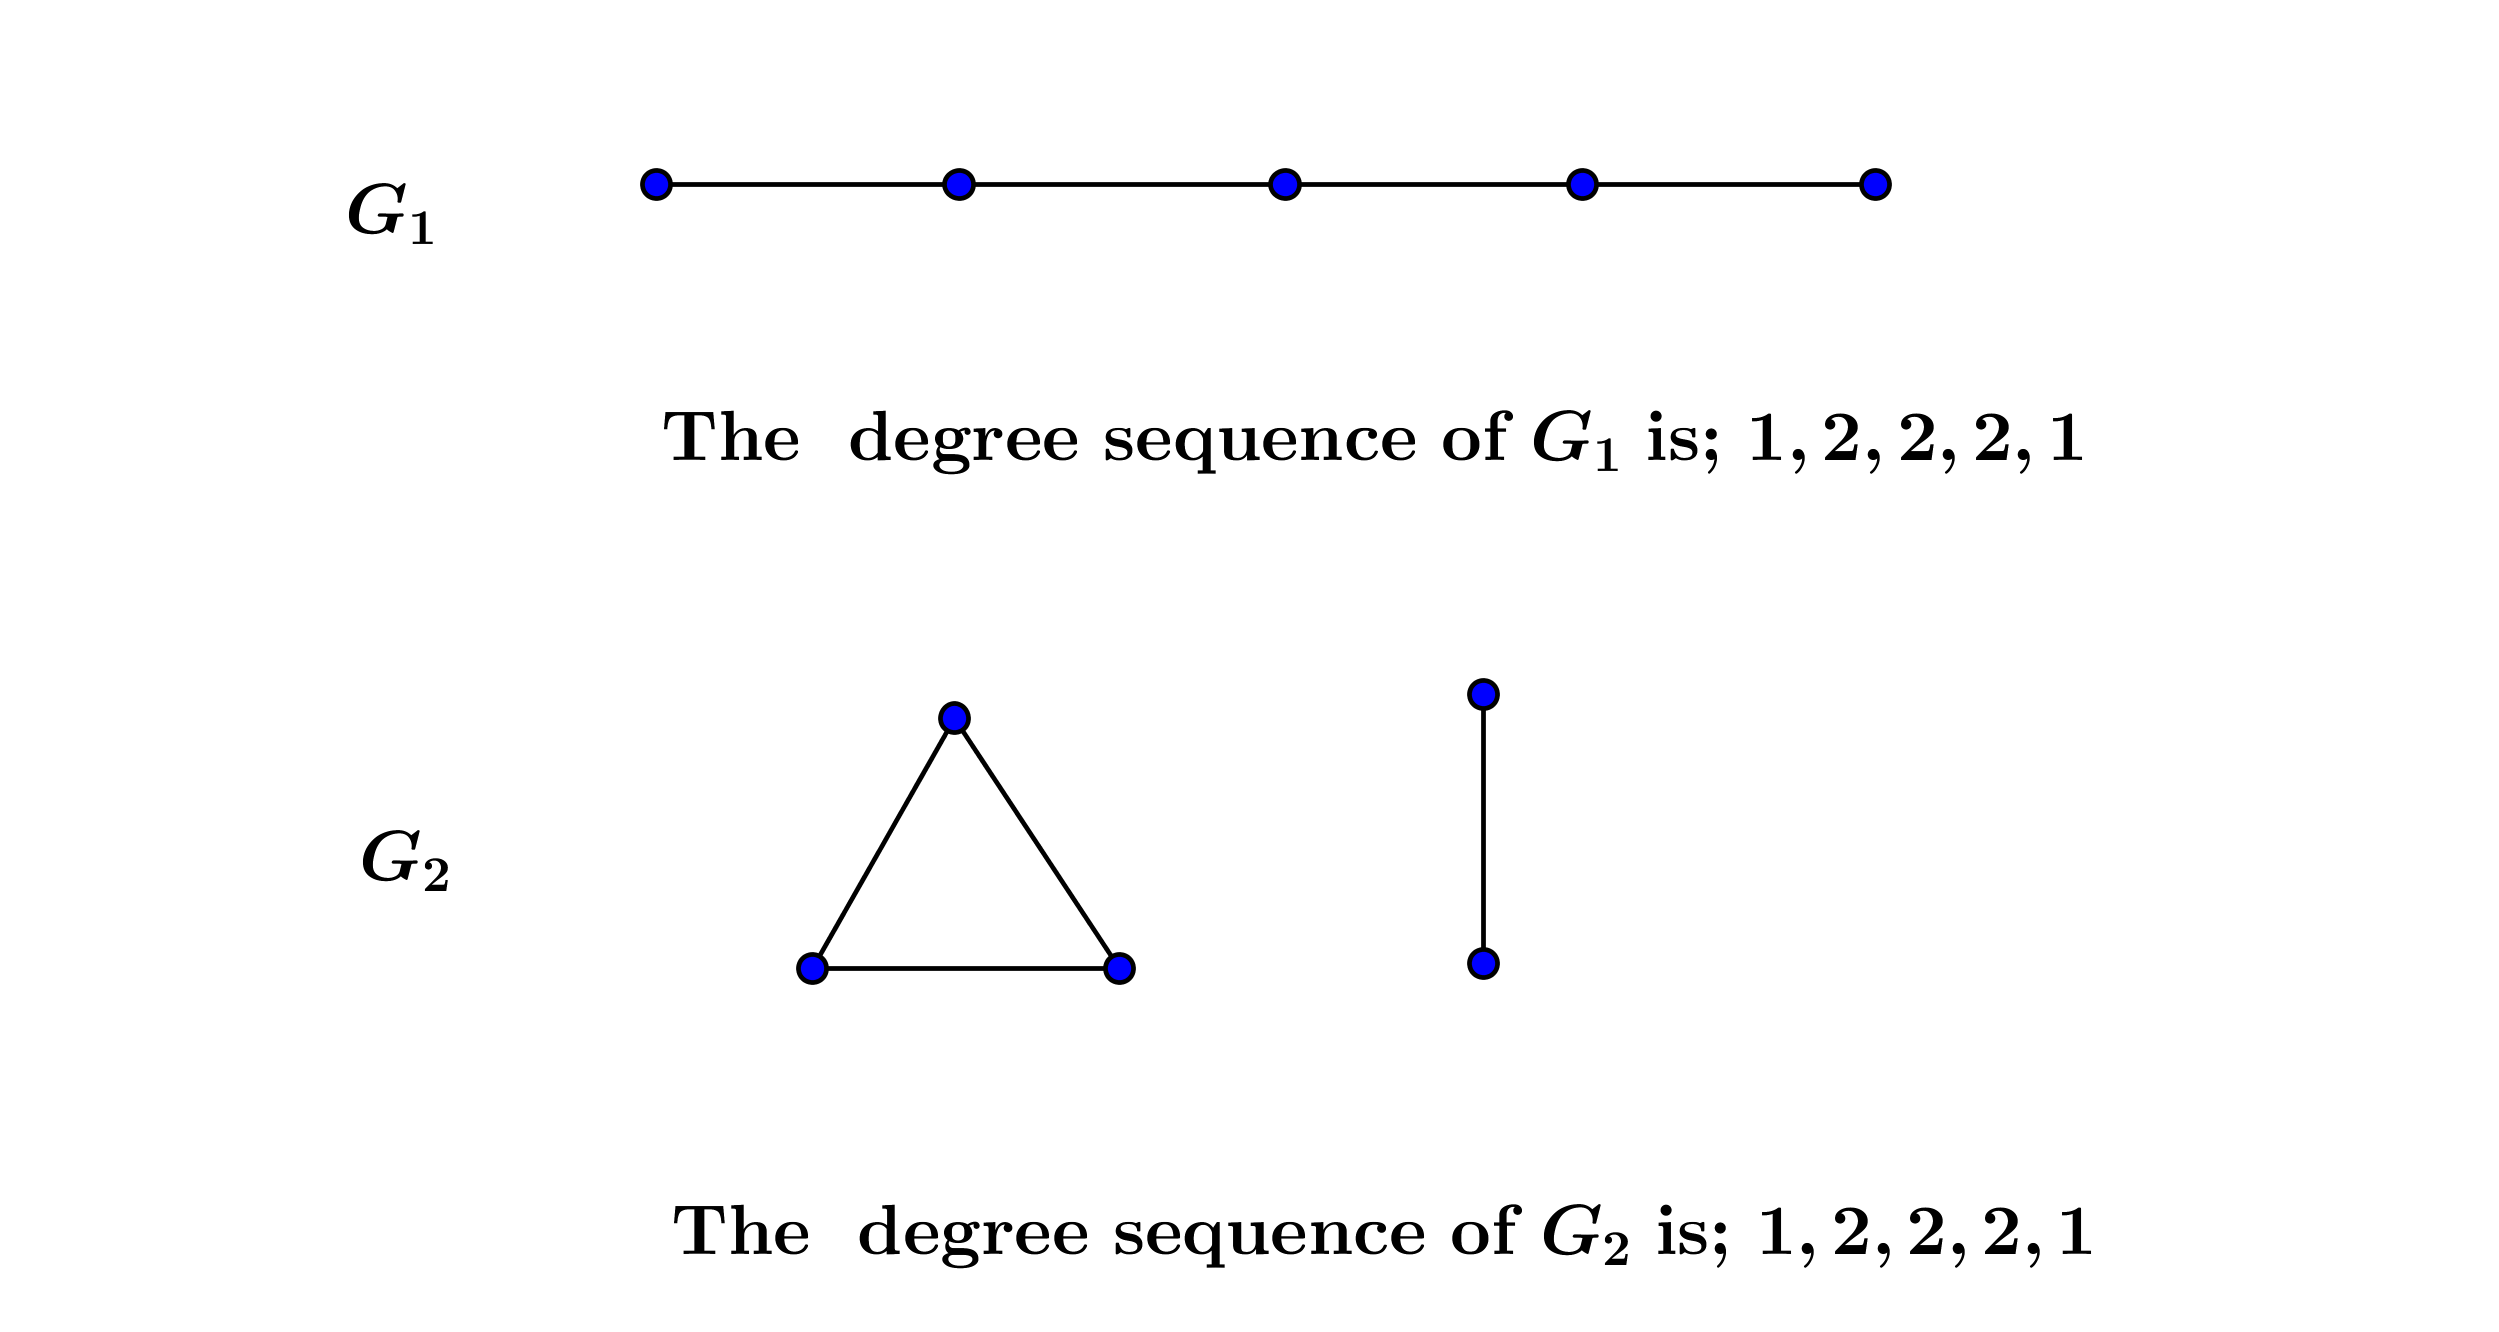
\includegraphics[width=.8\textwidth]{SolGrapg1g2.png}
\end{figure}
Hence $G_1$ and $G_2$ are non-isomorphic order 5 graphs of the same degree sequence.
\item $G_1$ and $G_2$ are isomorphic.
  \begin{figure}[hbt!]
\centering
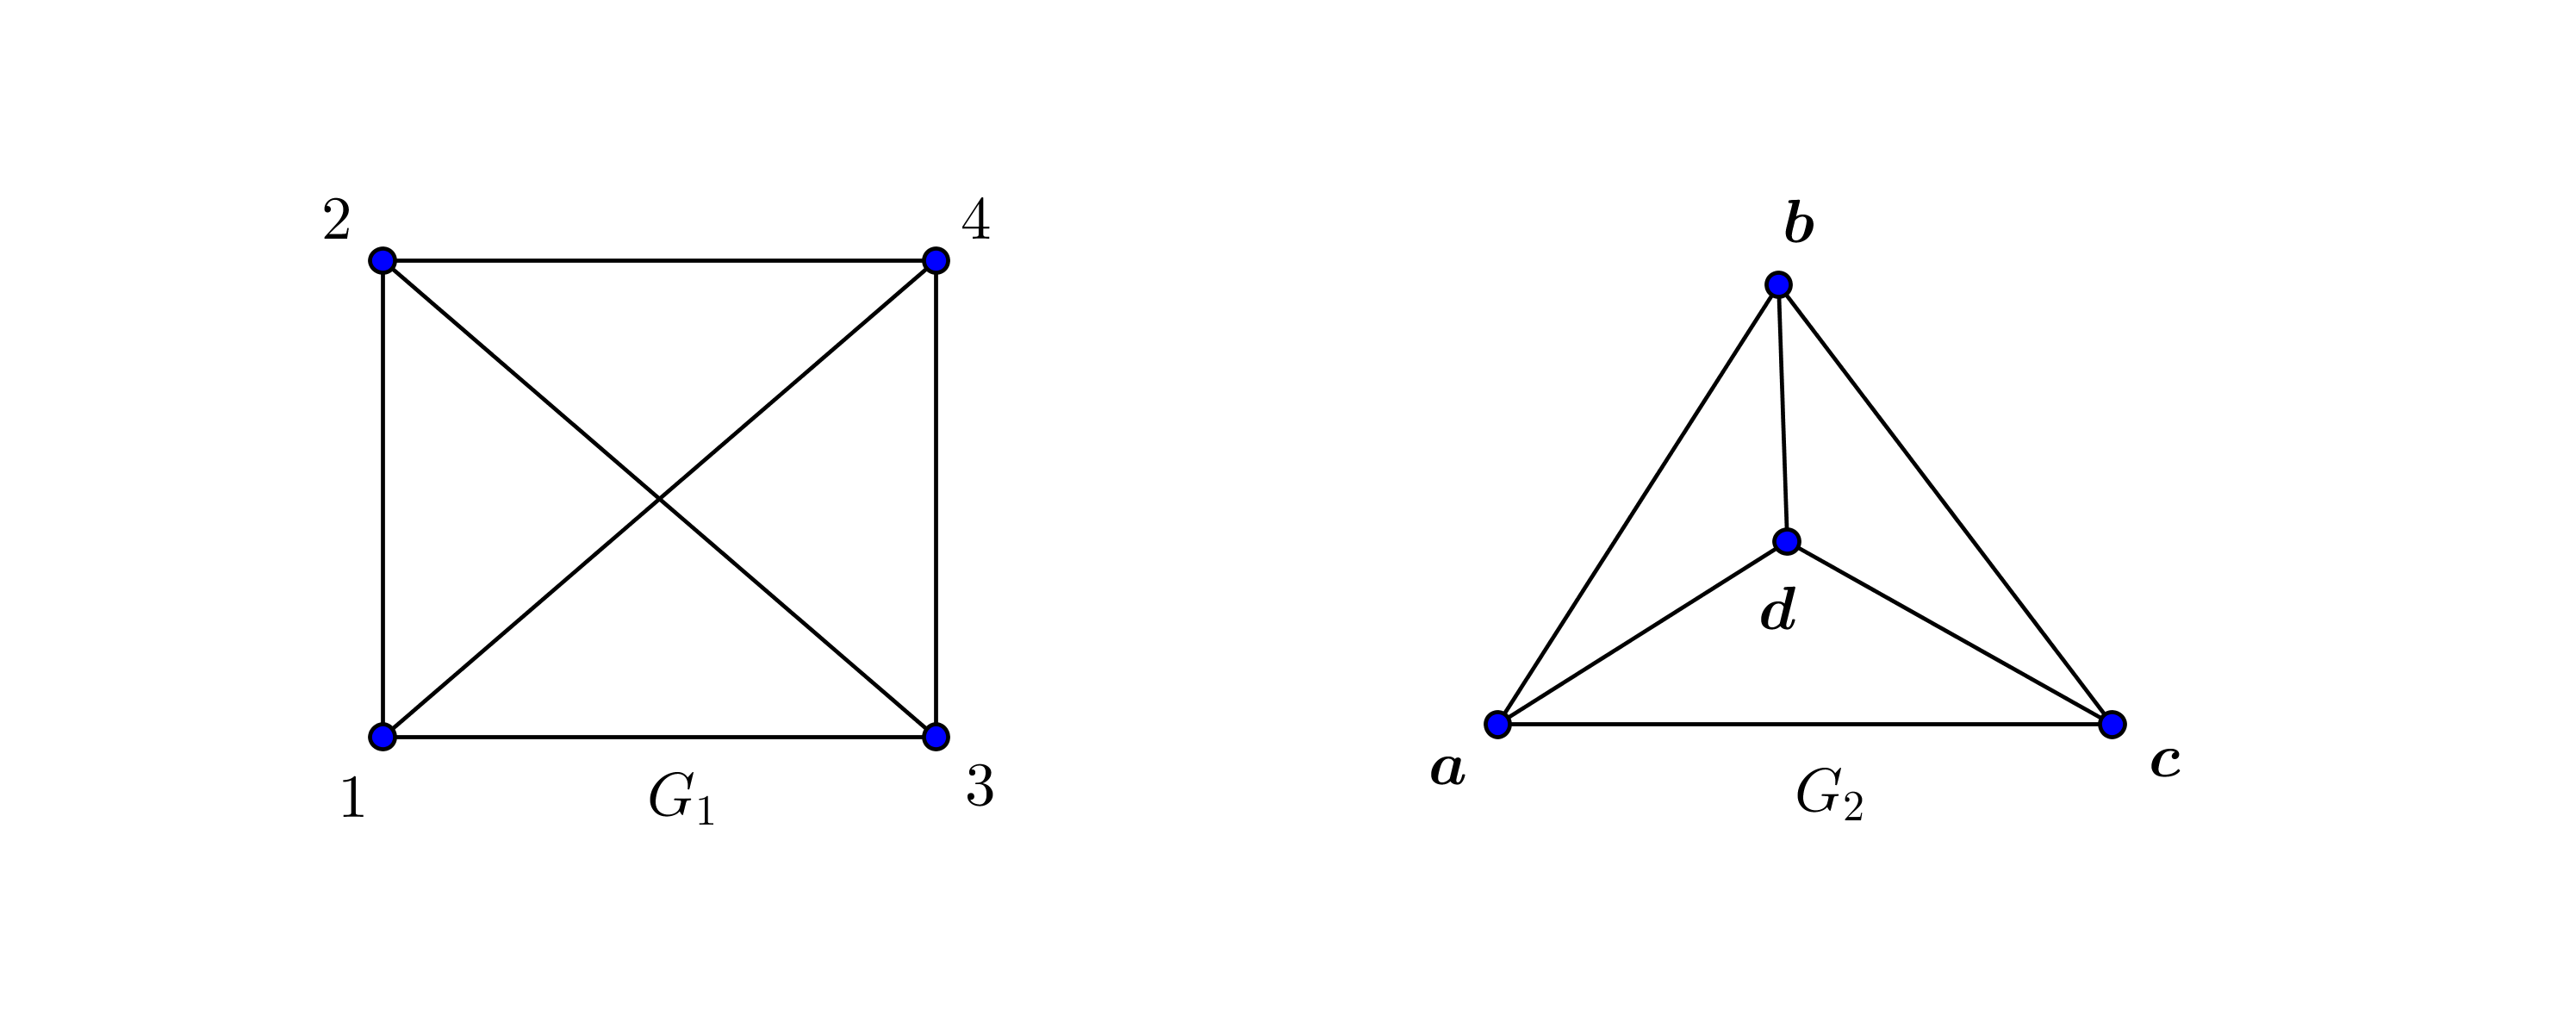
\includegraphics[width=.6\textwidth]{SolGrapAsse8a.png}
\end{figure}

  The isomorphism between $G_1$ and $G_2$ is the map
  $
  \{f: 1\mapsto a,2\mapsto b,3\mapsto c,4\mapsto d\}.
  $

  $G_3$ and $G_5$ are isomorphic.

  \begin{figure}[hbt!]
\centering
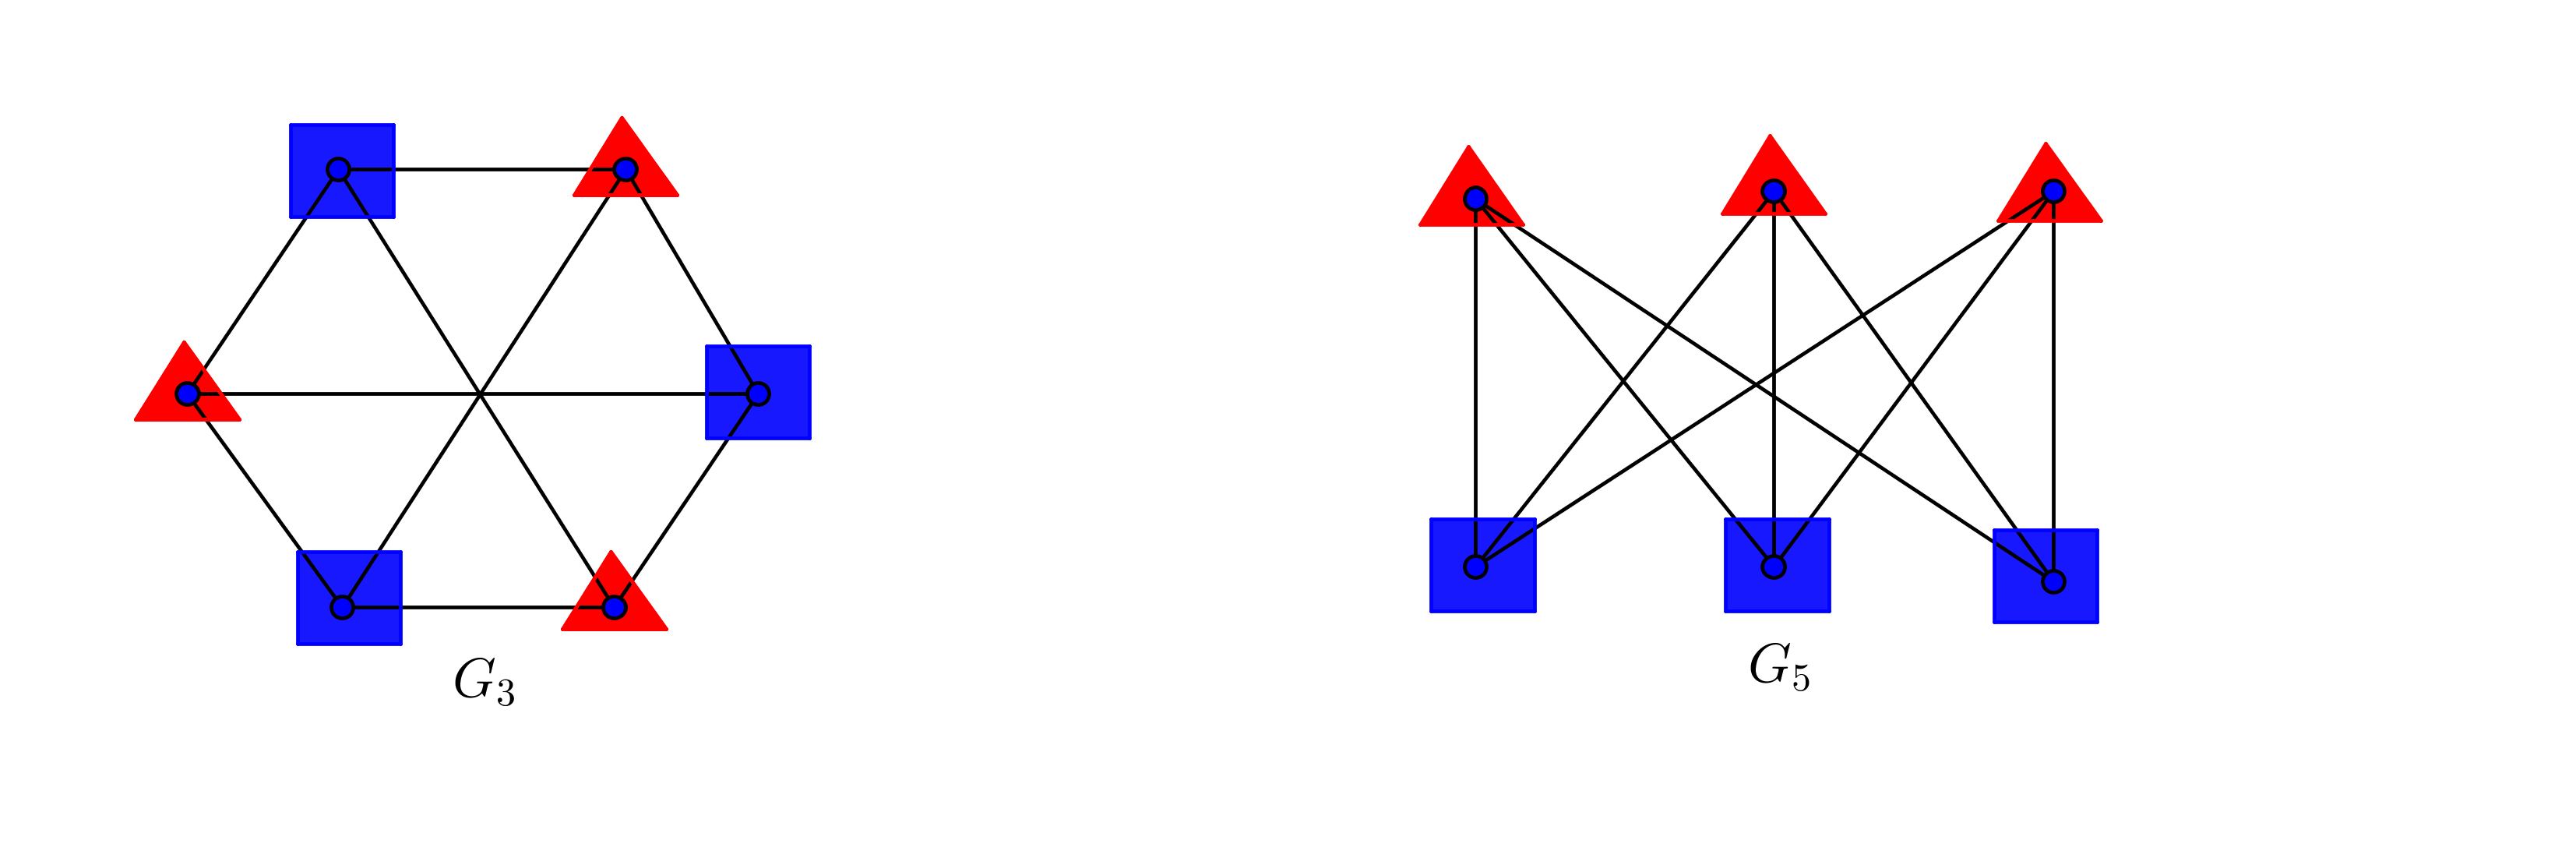
\includegraphics[width=.8\textwidth]{SolGrapAsse8b.png}
\end{figure}
\begin{align*}
  G_3\cong K_{3,3}\qquad &,\qquad K_{3,3}\cong G_5\\
  G_3&\cong G_5 \tag{since isomorphism is an equivalence relation}
  \end{align*}
\newpage
  \item (a)

  \begin{figure}[hbt!]
\centering
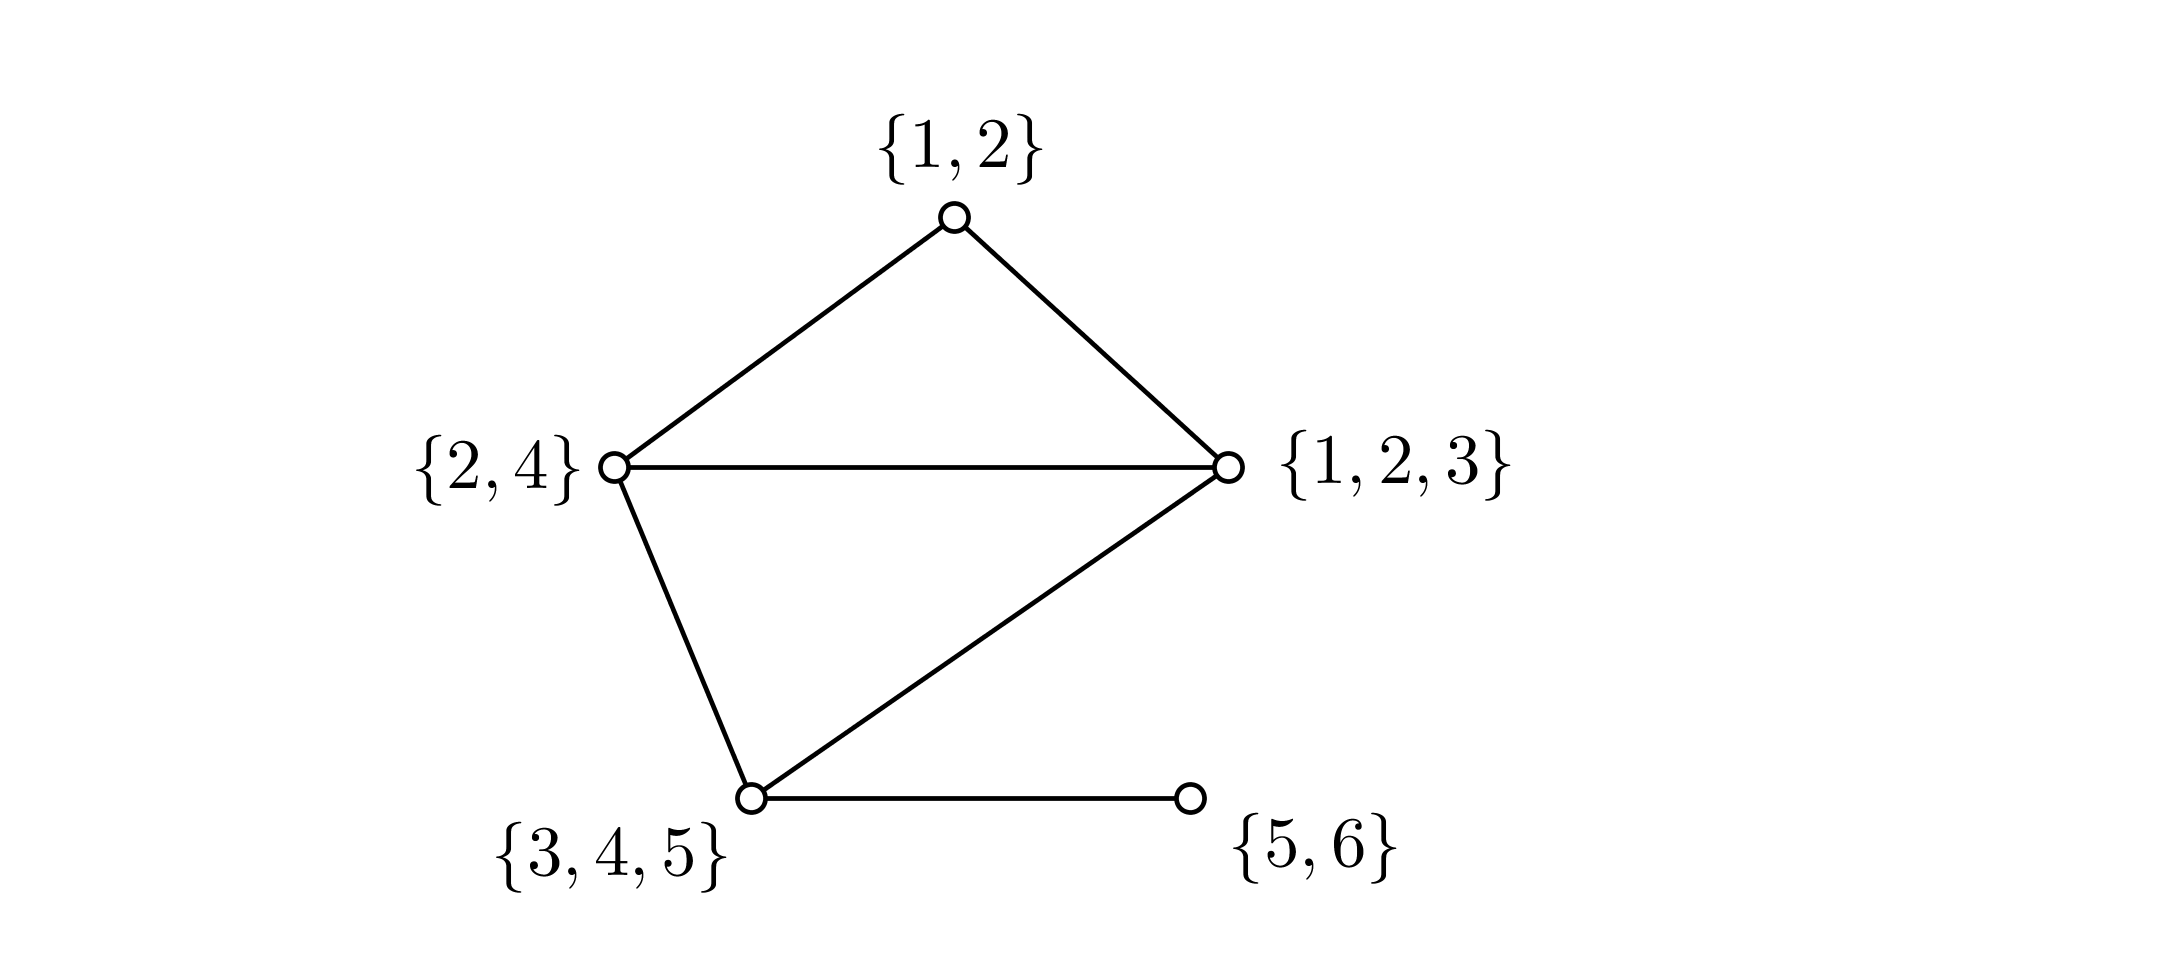
\includegraphics[width=.8\textwidth]{SolGrapAsse9a.png}
\end{figure}

  (b)

  \begin{figure}[hbt!]
\centering
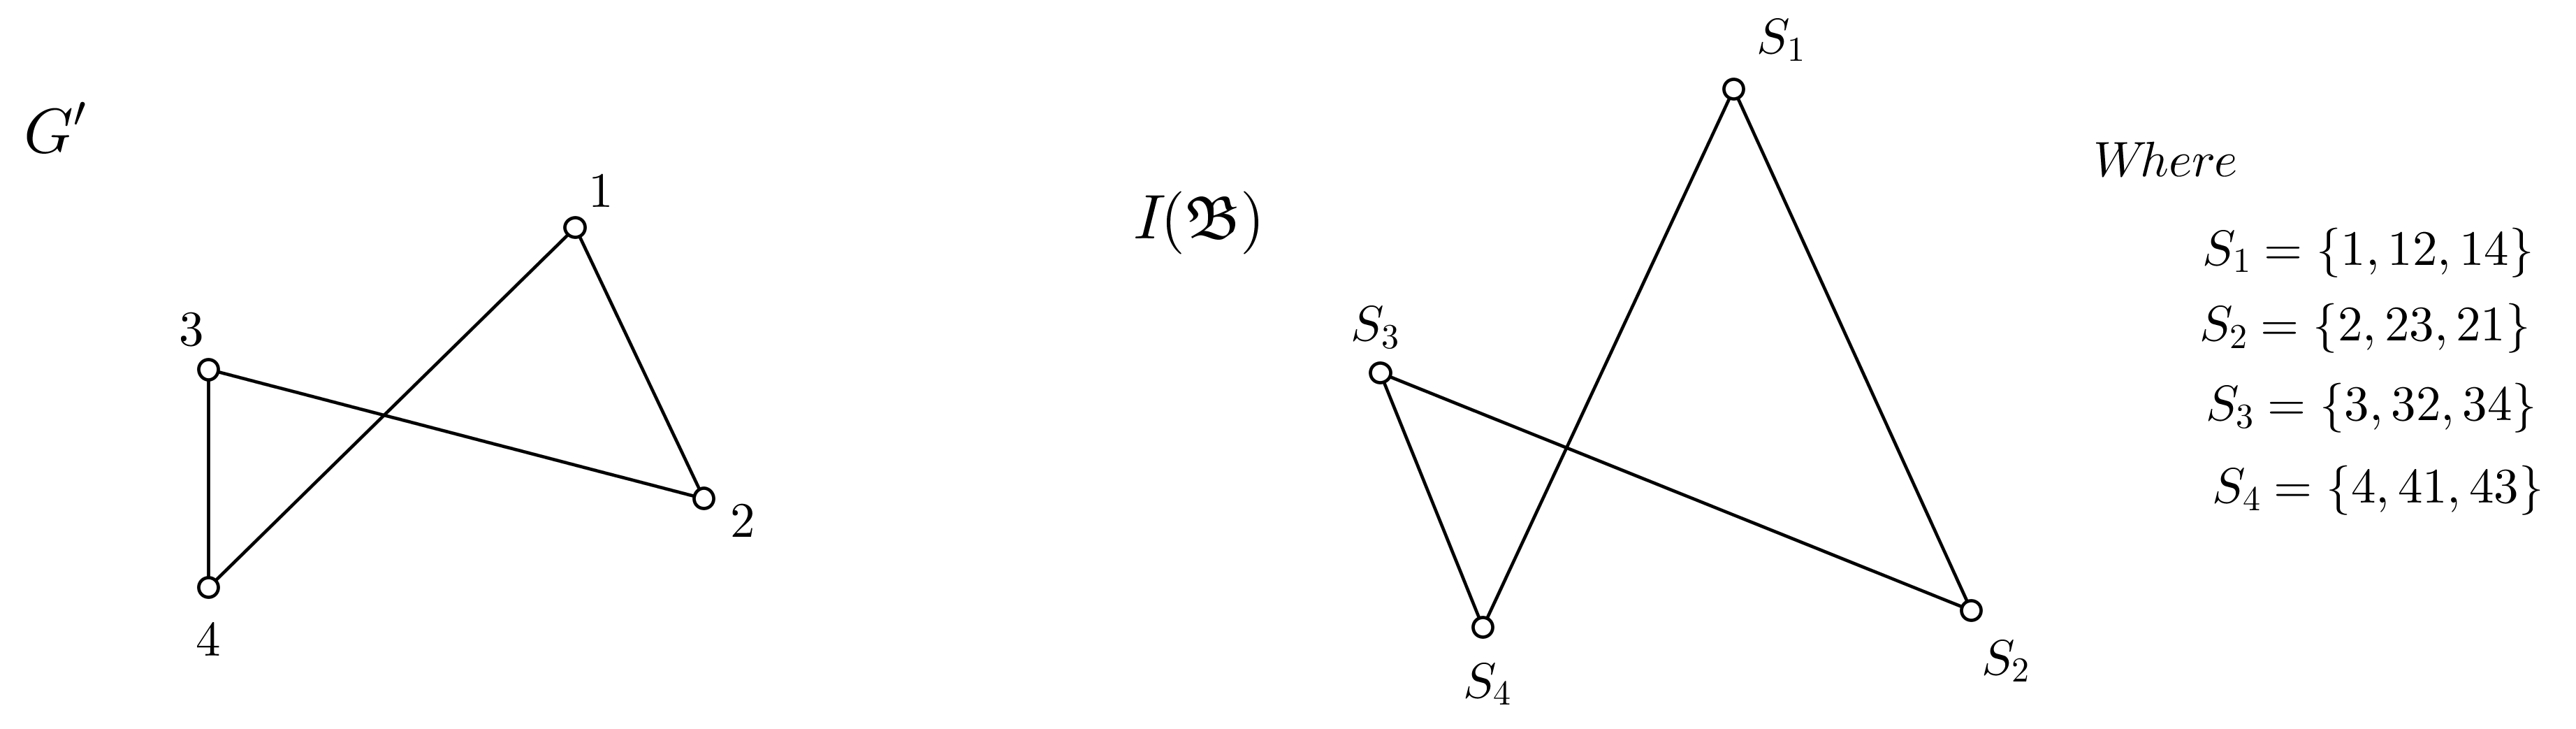
\includegraphics[width=1.0\textwidth]{SolGrapAsse9b.png}
\end{figure}

The isomorphism $I(\mathfrak{B})\rightarrow G'$ is given by $S_i\rightarrow i$ for $i=1,2,3,4$.

\item The simplest(the best) way to approach this problem is by using \textbf{Pigeonhole Principle}\footnote{Peter Gustav Lejeune Dirichlet ($1805 - 1859$).}.\\
So, assume components as hole and vertices as pigeon.\\
Now if we let each component to have $4$ vertices($4+4+4=12=13-1$), then we will left with one extra vertex. This extra vertex belongs to one of the three components(since we've only three components). But adding that extra vertex to any of the components results a component with $5$ vertices(since each component has already $4$ vertices).
$\Box$

  \item The minimum size of $G$ is
  $$
\begin{cases}
\frac{n}{2}\biggl( \frac{n-2}{2}\biggl),&\mbox{ for }n \text{ even.}\\
\medskip
\biggl( \frac{n-2}{2}\biggl)^2,&\mbox{ for }n \text{ odd.}
\end{cases}
$$
The maximum possible size of $G$ is
$$
\frac{(n-2)(n-1)}{2}
$$
\newpage
  \item Removing just one vertex $d$ results disconnection in both graph (a) and (b).

  \begin{figure}[hbt!]
\centering
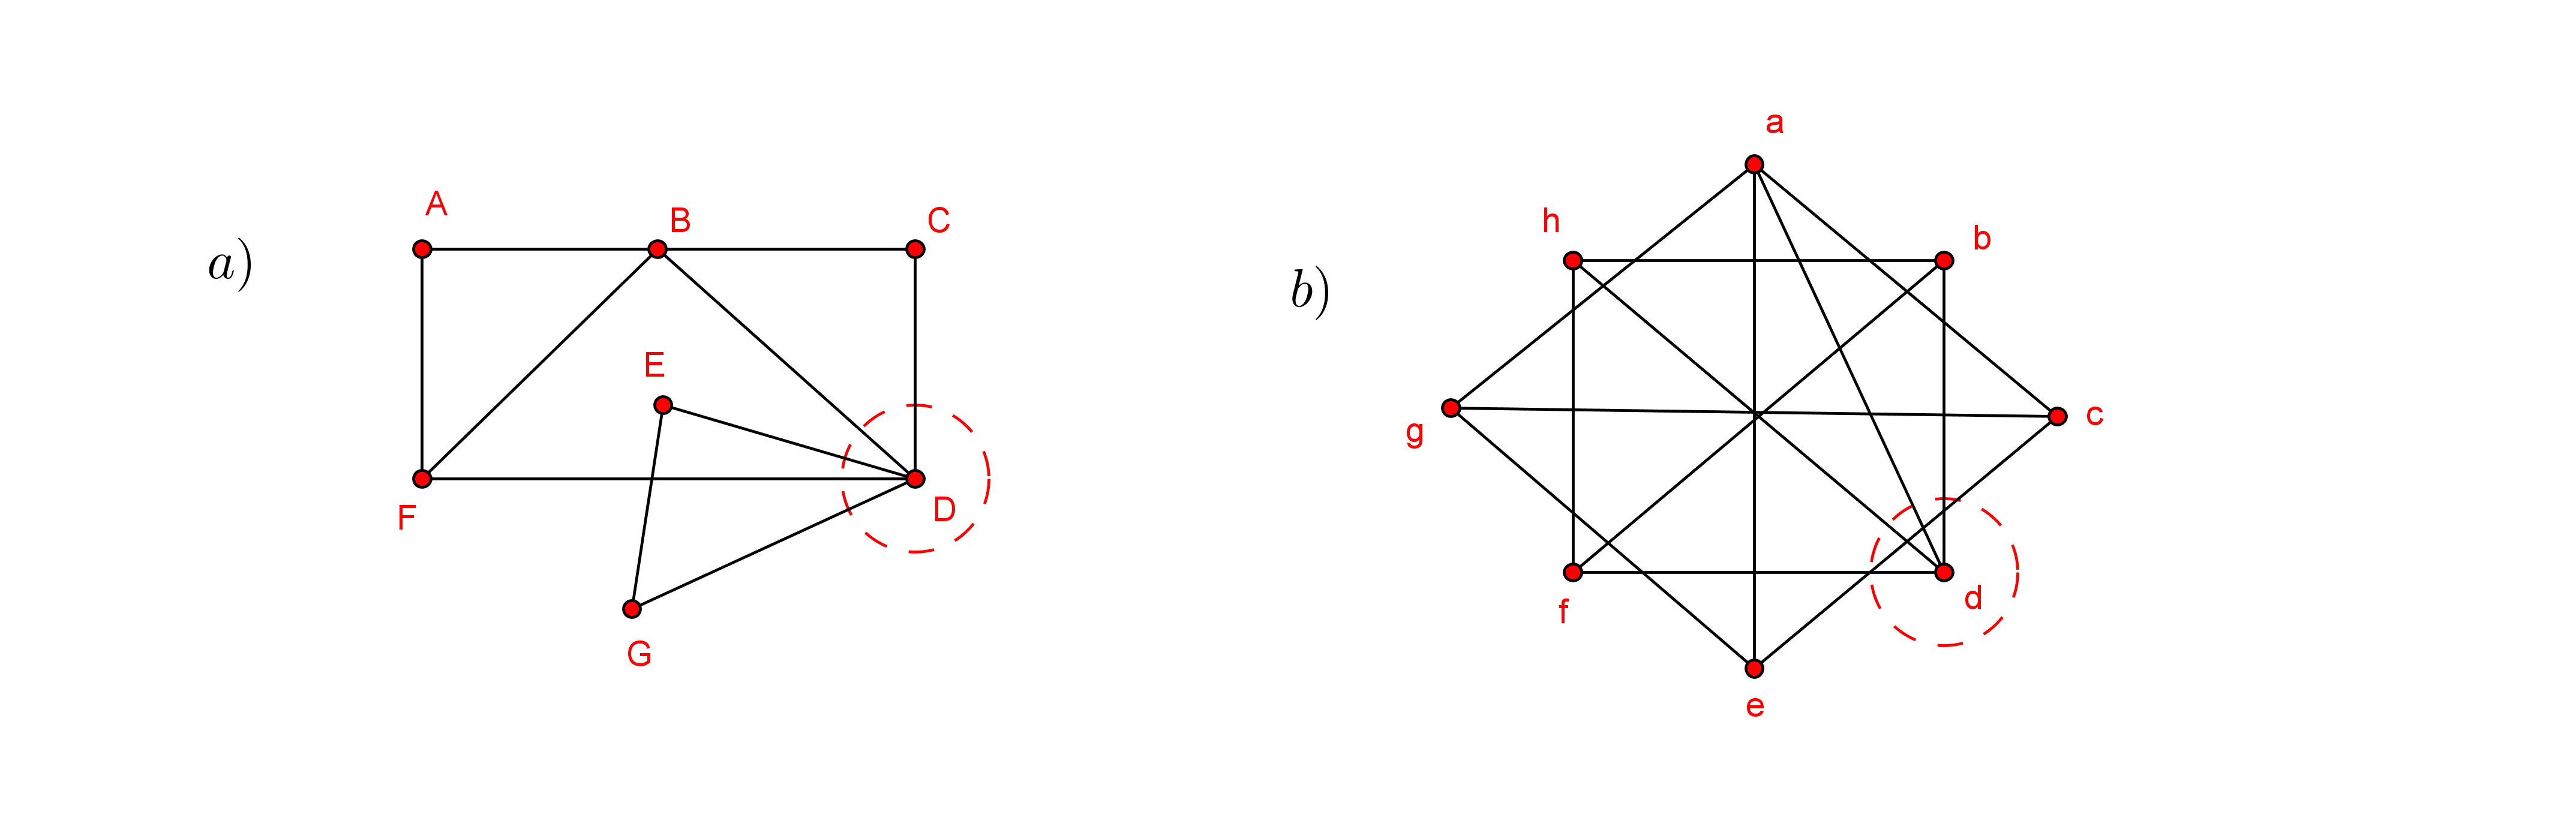
\includegraphics[width=1.0\textwidth]{SolGrapAss2.png}
\end{figure}

  \item (a)

   \begin{figure}[hbt!]
\centering
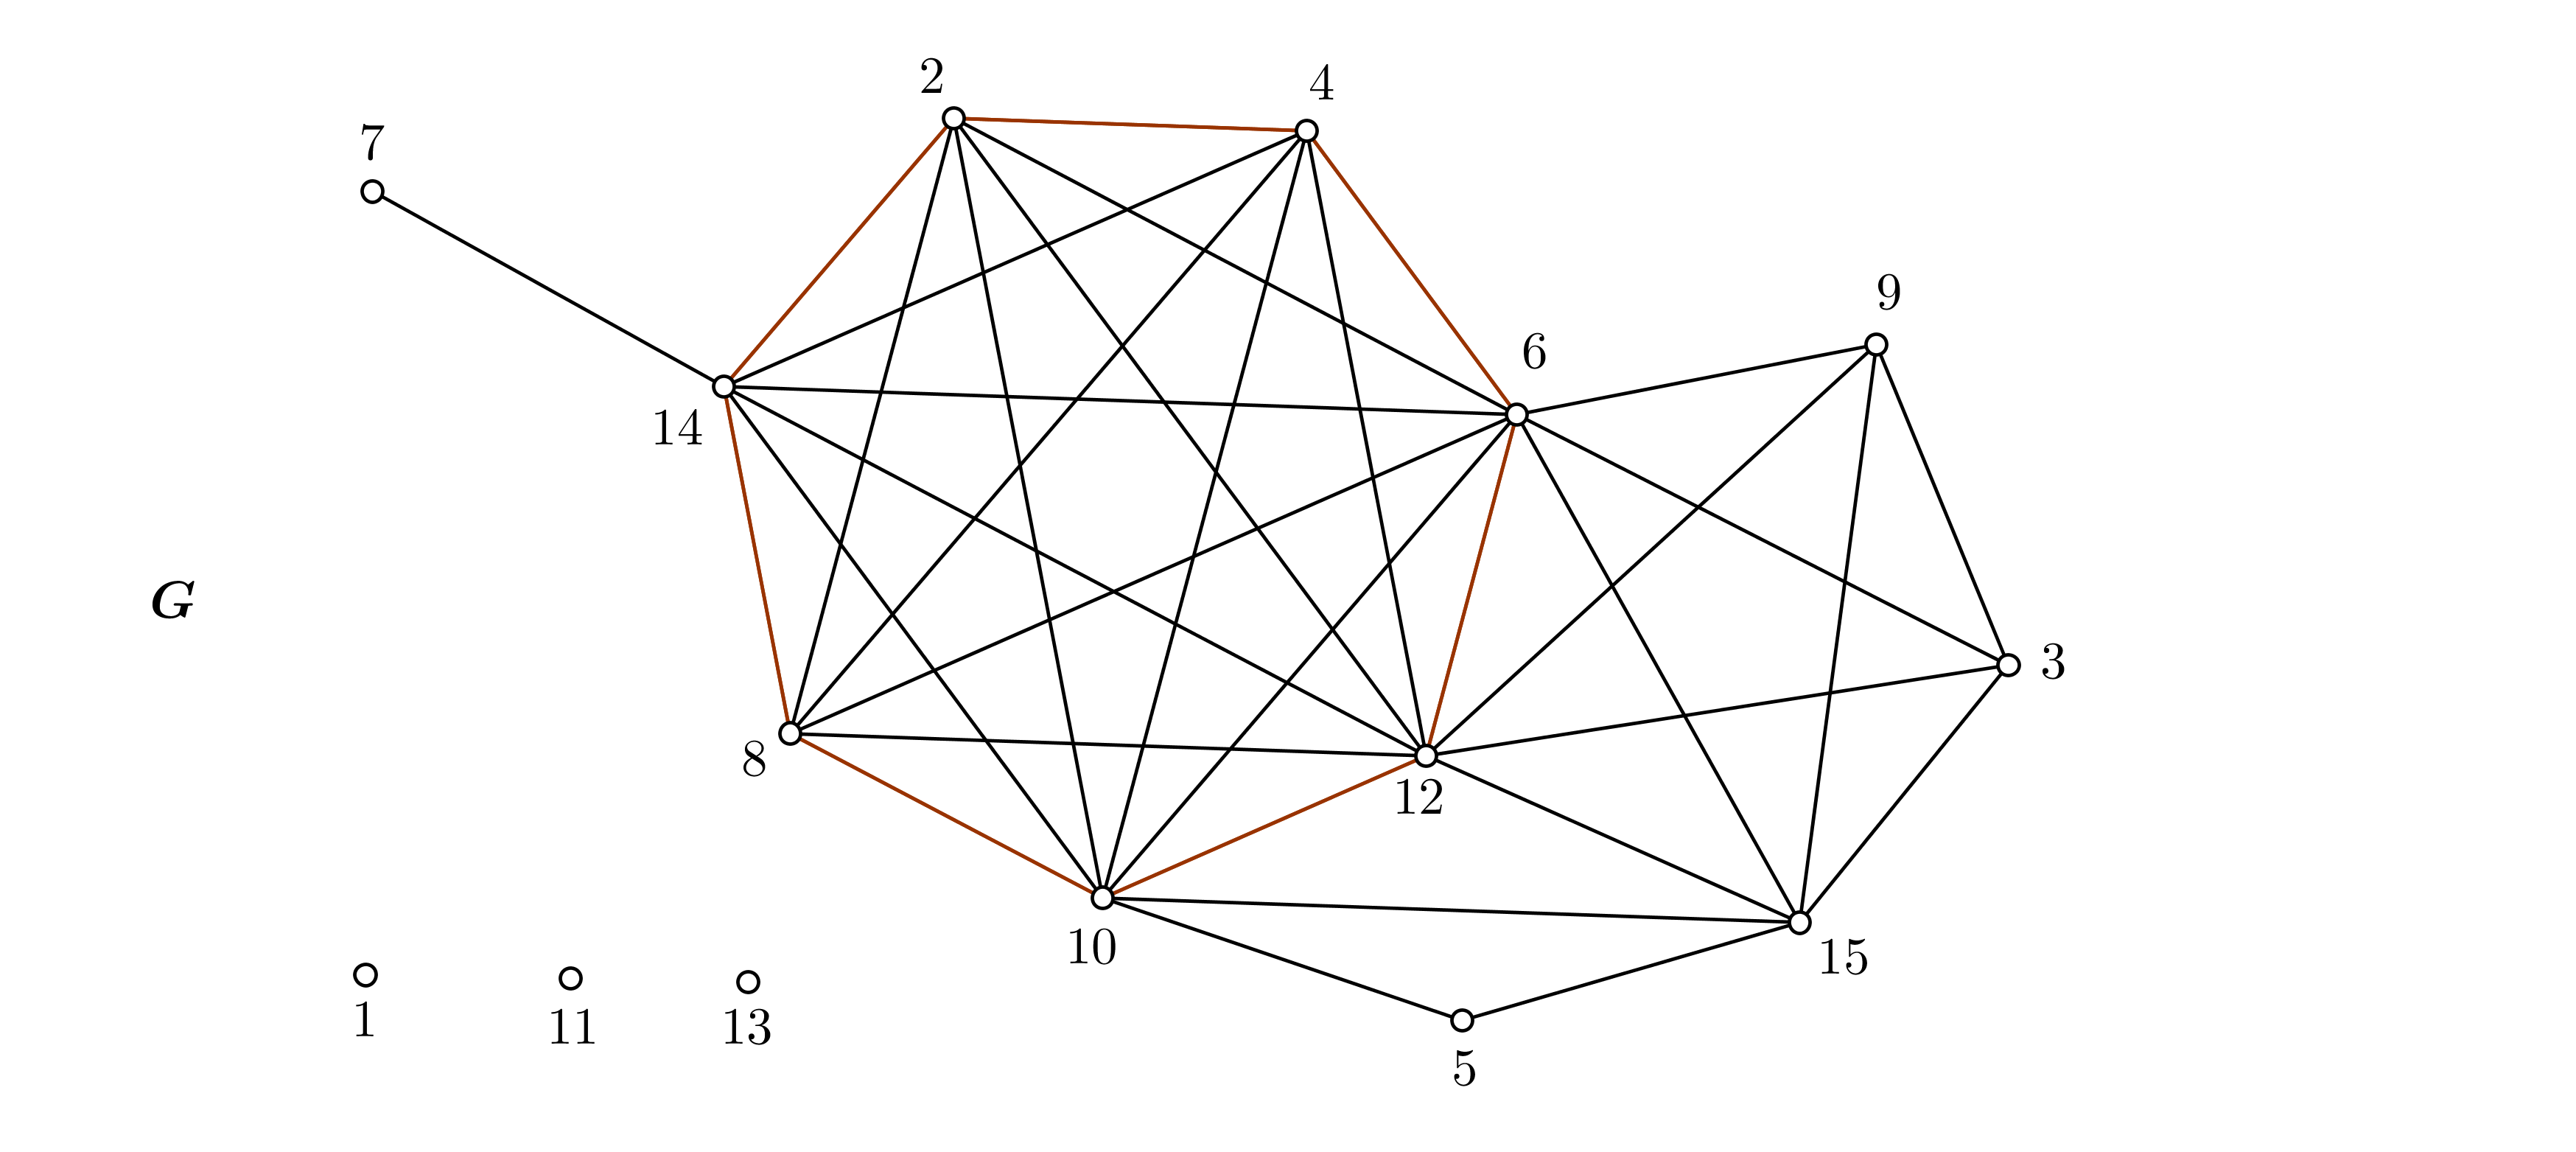
\includegraphics[width=1.0\textwidth]{SolGrapAsse13a.png}
\end{figure}

  (b) The longest path in $G$ is of length $11$.

  \item diam($G$) to say diameter of $G$

  \begin{align*}
  \text{(1) diam(peterson)}&=2\qquad \text{(4) diam($K_{n,m}$)}=\begin{cases}
1,&\mbox{ for }n=m=1\\
\medskip
2,&\mbox{ otherwise.}
\end{cases}\\
  \text{(2) diam($Q_n$)}&=n \qquad \text{(5) diam($C_n$)}=\biggl\lfloor\frac{n}{2}\biggl\rfloor\\
  \text{(3) diam($K_n$)}&=1 \qquad \text{(6) diam($P_n$)}=n-1
  \end{align*}
  \newpage
  \item None of them are Hamiltonian. None of them are Eulerian except (iii).

  \begin{figure}[hbt!]
\centering
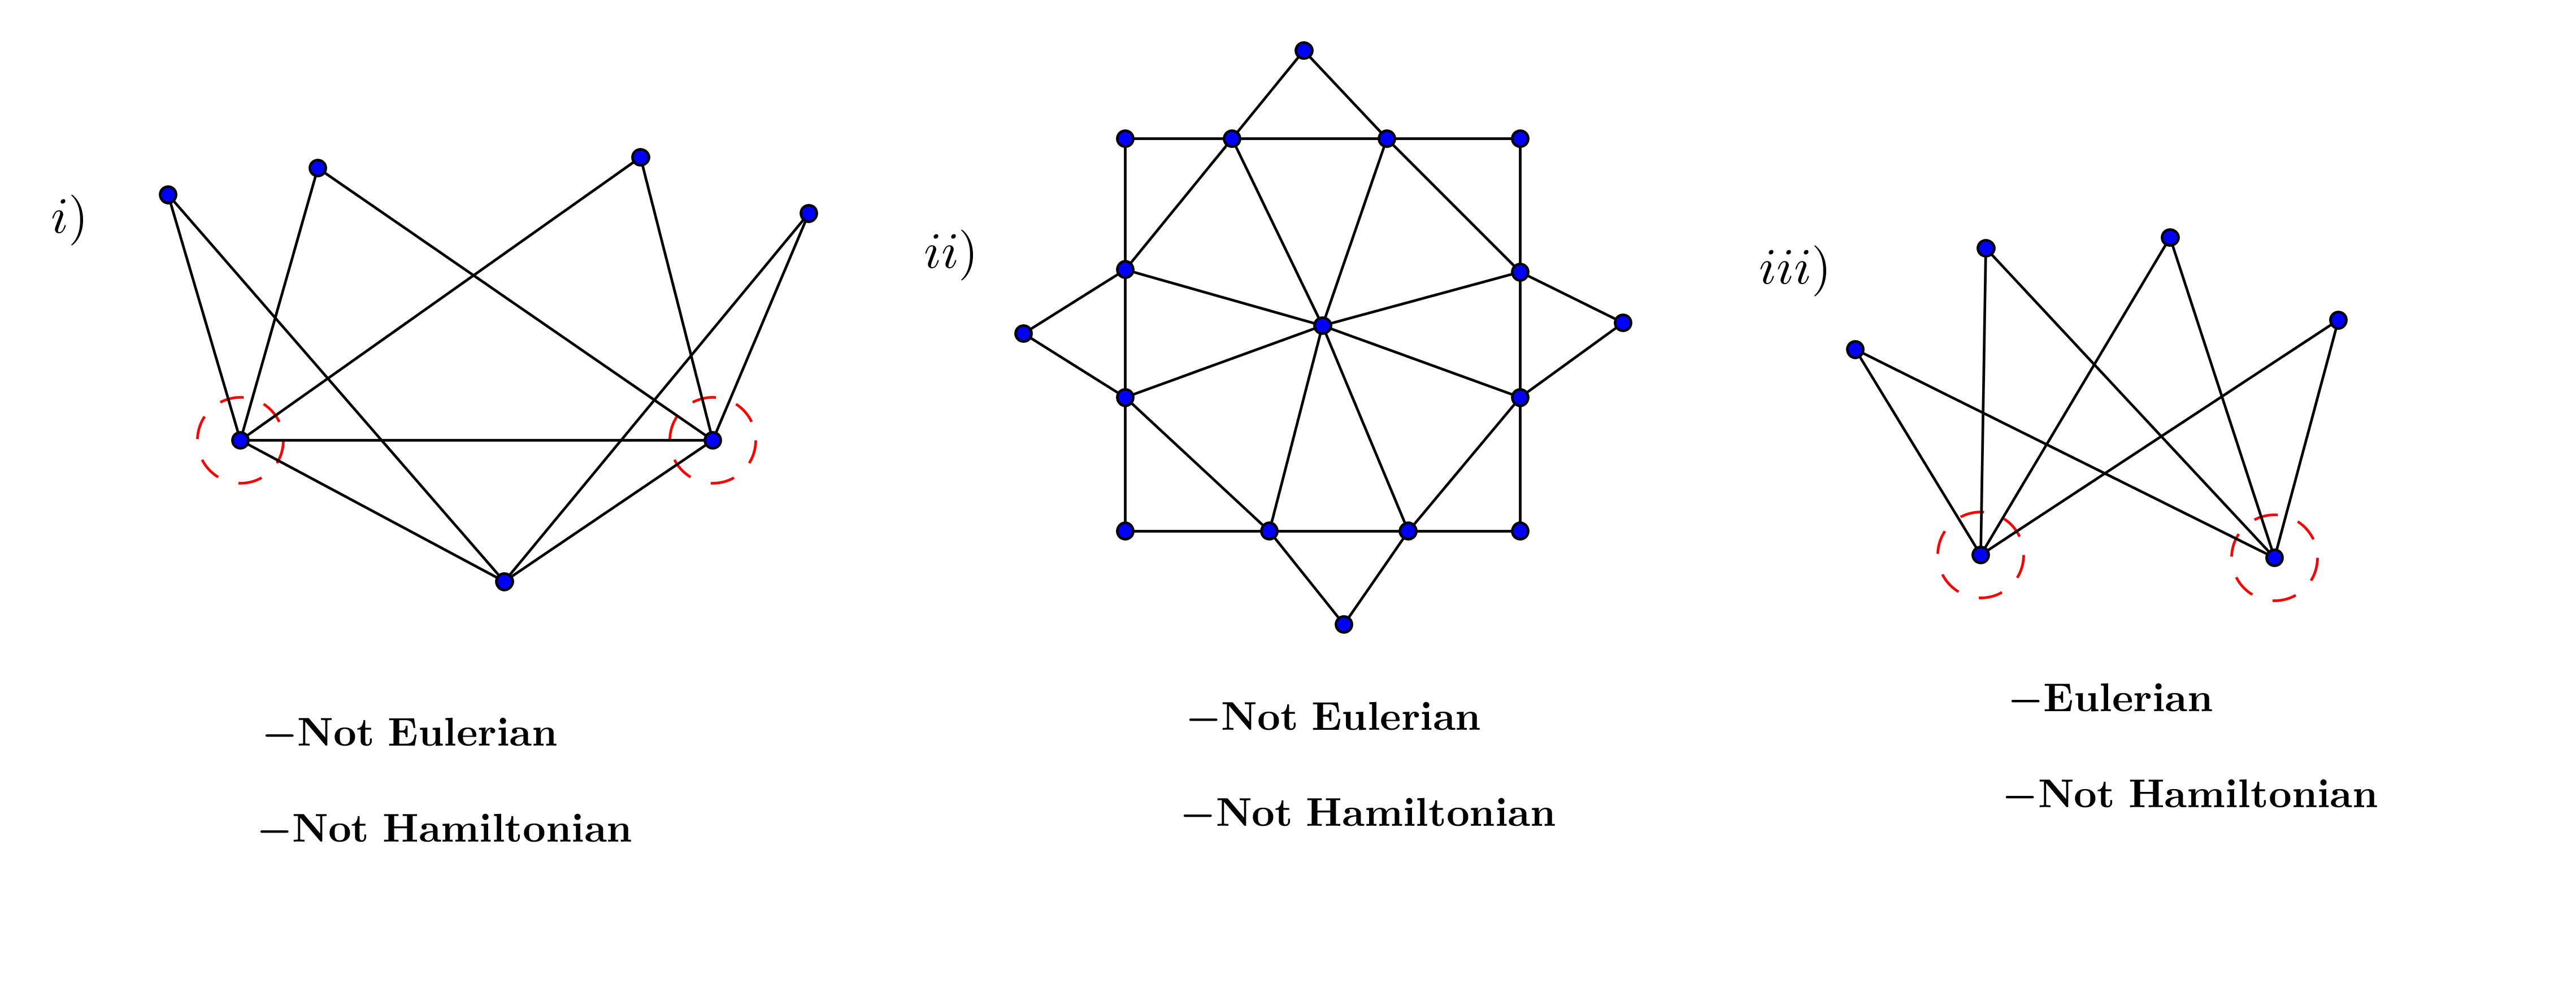
\includegraphics[width=1.0\textwidth]{SolGrapAss3.png}
\end{figure}

  \item Let $G$ be a regular graph with even order and odd size.
  \begin{align*}
  |G|=m\text{-even}.\\
  \|G\|=n\text{-odd}.
  \end{align*}
  Since $G$ is regular the degree of each vertex is the same, say $k$. \\
  WTS:- $k$ is odd, hence non Eulerian follows.\\
  Now
  \begin{align*}
  \sum_{v\in V(G)}\deg(v)=k\cdot\underbrace{m}_{even}=2\|G\|=2\cdot\underbrace{n}_{odd}
  \end{align*}
  \begin{align}\label{eusta}
  \Rightarrow k\biggl(\frac{m}{2}\biggl)=\underbrace{n}_{odd}
  \end{align}
  Since $m$ is even, $\frac{m}{2}\in \mathbb{Z}^{+}$, and we know that $k\in \mathbb{Z}^{+}$.\\
  From (\ref{eusta}), we have the product of two integers resulting an odd number $n$.\\
  Thus both $k$ and $\frac{m}{2}$ must be odd. Hence the degree of each vertex in $G$ is odd.\\
  Therefore, $G$ is not Eulerian.$\Box$

  \item Let's put vertices on the drawings and imagine as they are graphs.

  \begin{figure}[hbt!]
\centering
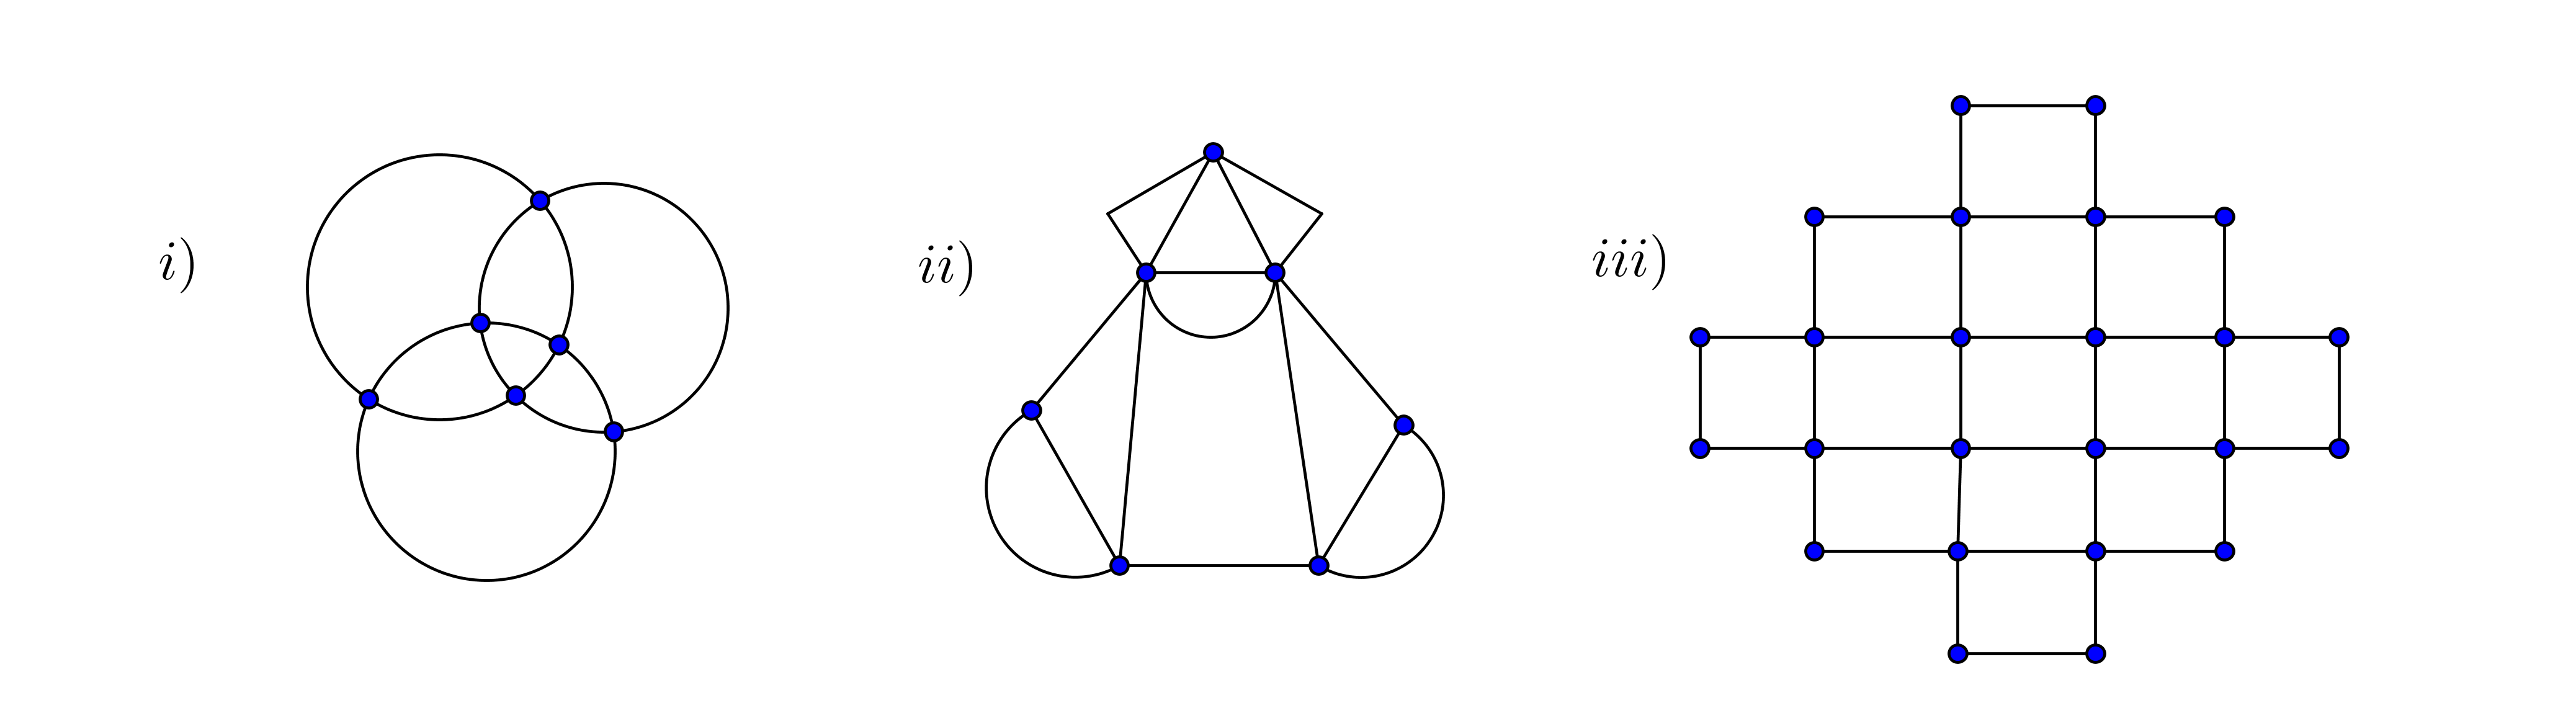
\includegraphics[width=1.0\textwidth]{SolGrapAss4.png}
\end{figure}

  There is an \textbf{Euler tour} in (i) and (iii) since every vertex is of even degree.\\
  Thus, the drawings in (i) and (iii) can be drawn without lifting one's pen from the paper and without repeating any line.
  (ii) also can be drawn in the same manner since there is an \textbf{Euler trail} that starts at $a$ and ends at $b$(vise versa).
  \newpage
  \item (a) Since $n=6$ the values of $m$ are $1$ and $2$.\\
  For $m=1$


  \begin{figure}[hbt!]
\centering
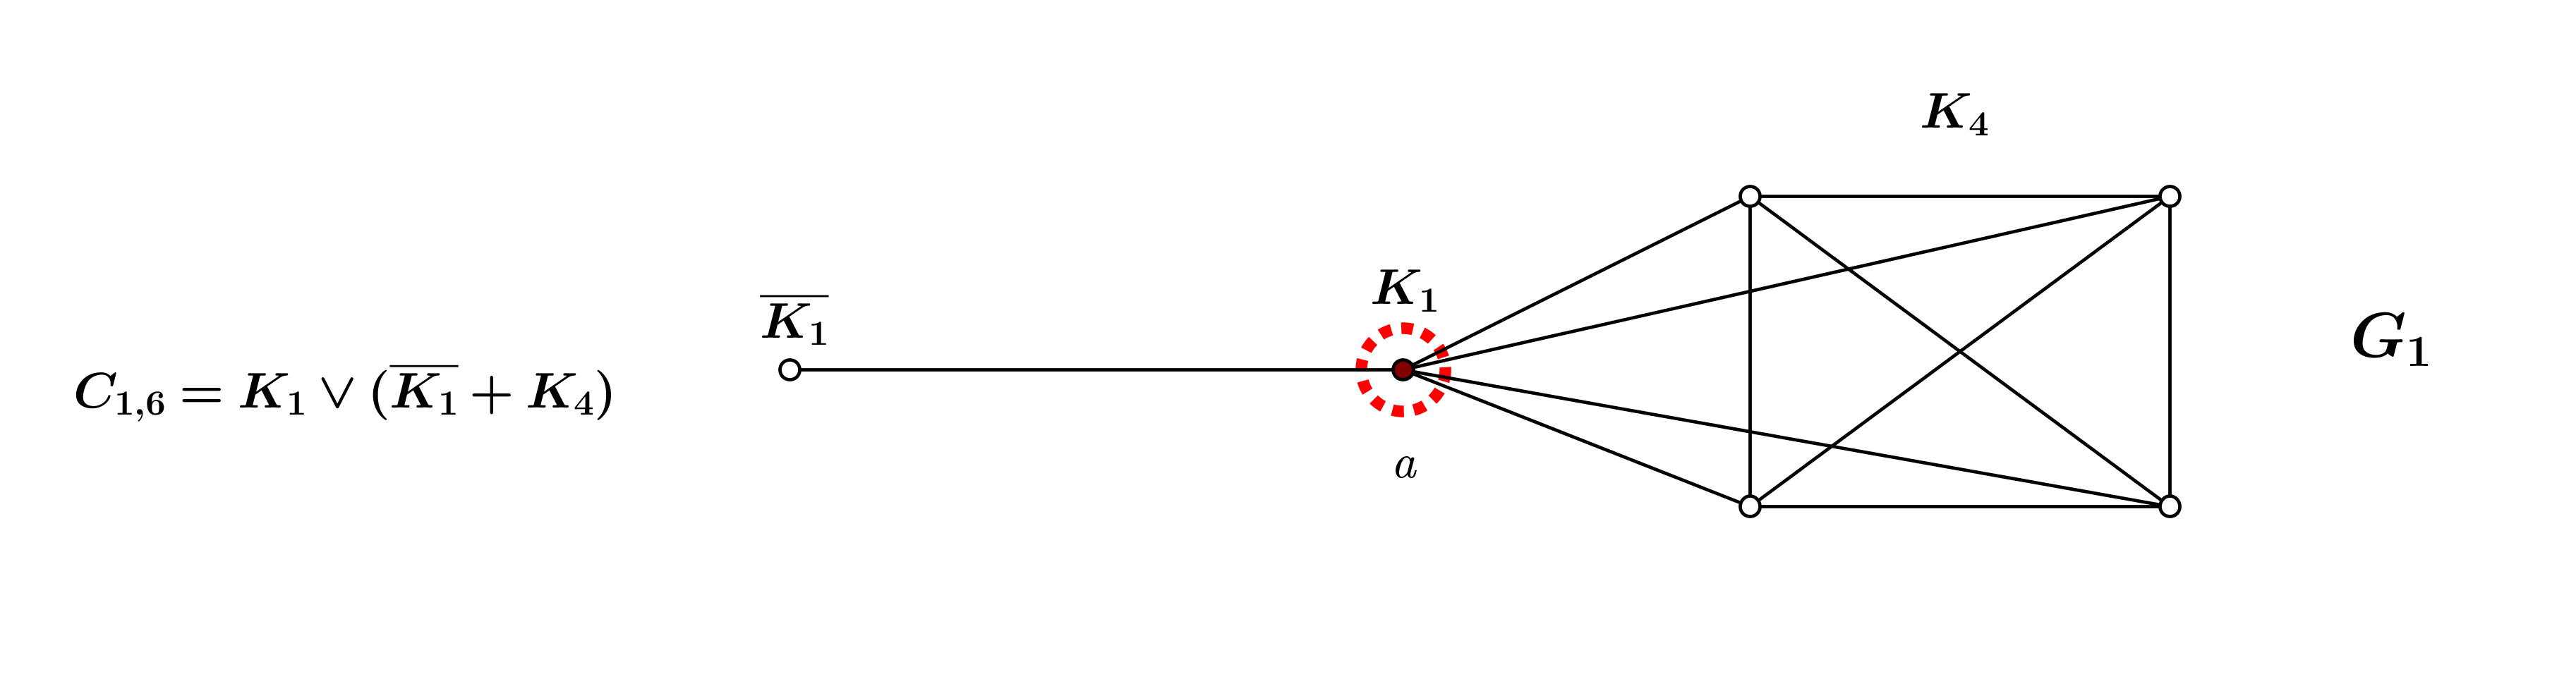
\includegraphics[width=1.0\textwidth]{SolGrapAssp2a.png}
\end{figure}

  For $m=2$,

  \begin{figure}[hbt!]
\centering
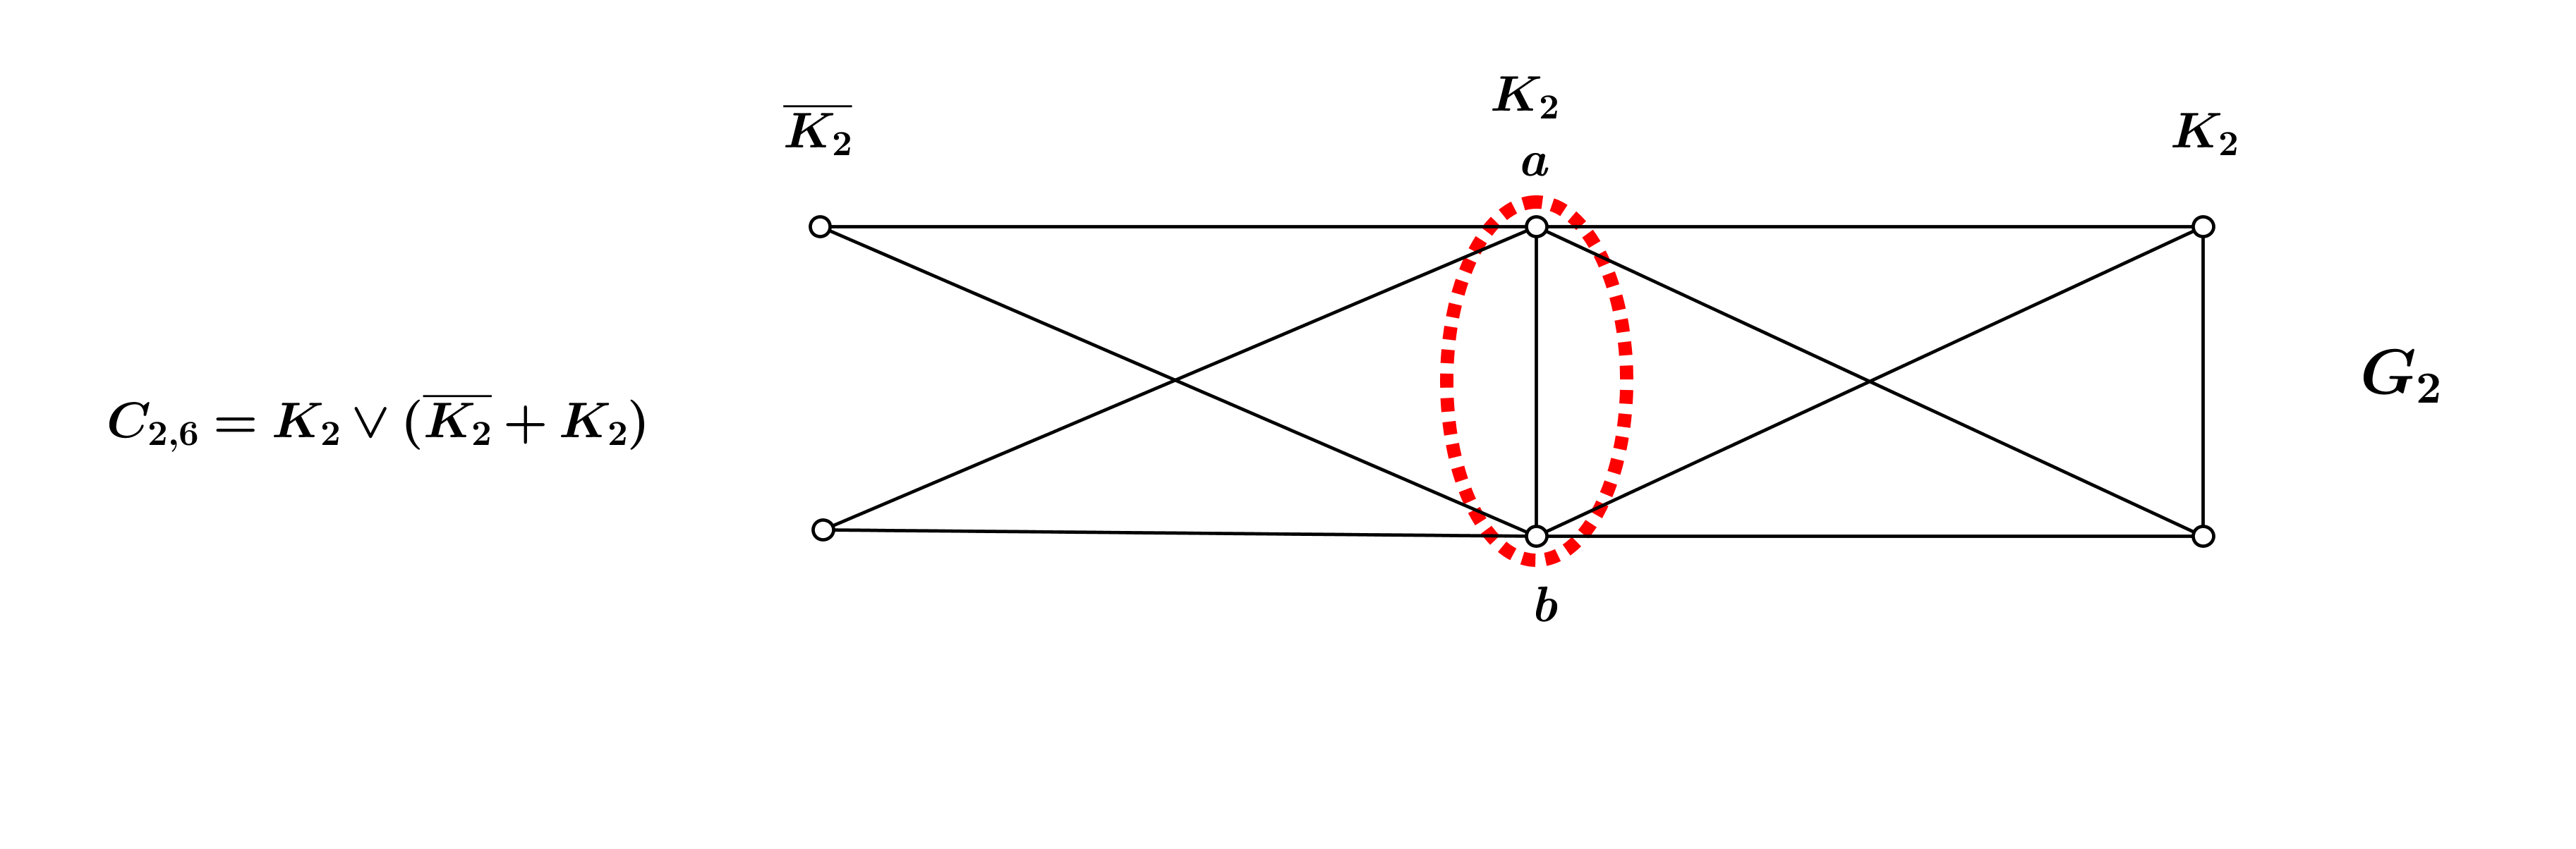
\includegraphics[width=1.0\textwidth]{SolGrapAssp2a1.png}
\end{figure}

  (b) The above $G_1$ and $G_2$ can't be Hamiltonian. Because removing the indicated vertices in \textcolor{red}{red} will result the number of component that exceed the number of vertices, which we've just removed. i.e. For $G_1$, take $S=\{a\}$\\
  \begin{align*}
  \Rightarrow |\omega(G_1-S)|=2\geq|S|=1
  \end{align*}
  For $G_2$, take $S=\{a,b\}$
  \begin{align*}
  \Rightarrow|\omega(G_2-S)|=3\geq2=|S|
  \end{align*}
  (c) The degree sequence of $G_1$ is; $1,4,4,4,4,5$ and \\
  The degree sequence of $G_2$ is; $5,5,3,3,2,2$\\
  (d) NO! It's impossible(Because of Chvatal's Theorem).

  \item The minimum number of edges in a simple graph of order $n\geq2$ that guarantee Hamiltonian is
  \begin{align*}
  \binom{n-1}{2}+2
  \end{align*}
  \item $\underbrace{n-2,n-2,\ldots,n-2}_{(n-2) \text{ times}},n-1,1$ is the degree of non-Hamiltonian simple graph with $n$ vertices and $\binom{n-1}{2}+1$ edges.
  \item $4,3,3,3,2,1,1,1,1,1,1,1$ is the degree sequence of the given tree.
  \newpage

  \item The sequence $7,2,2,1,1,1,1,1,1,1$ is the degree sequence of tree because we have found one. Look at the tree below
  \begin{figure}[hbt!]
\centering
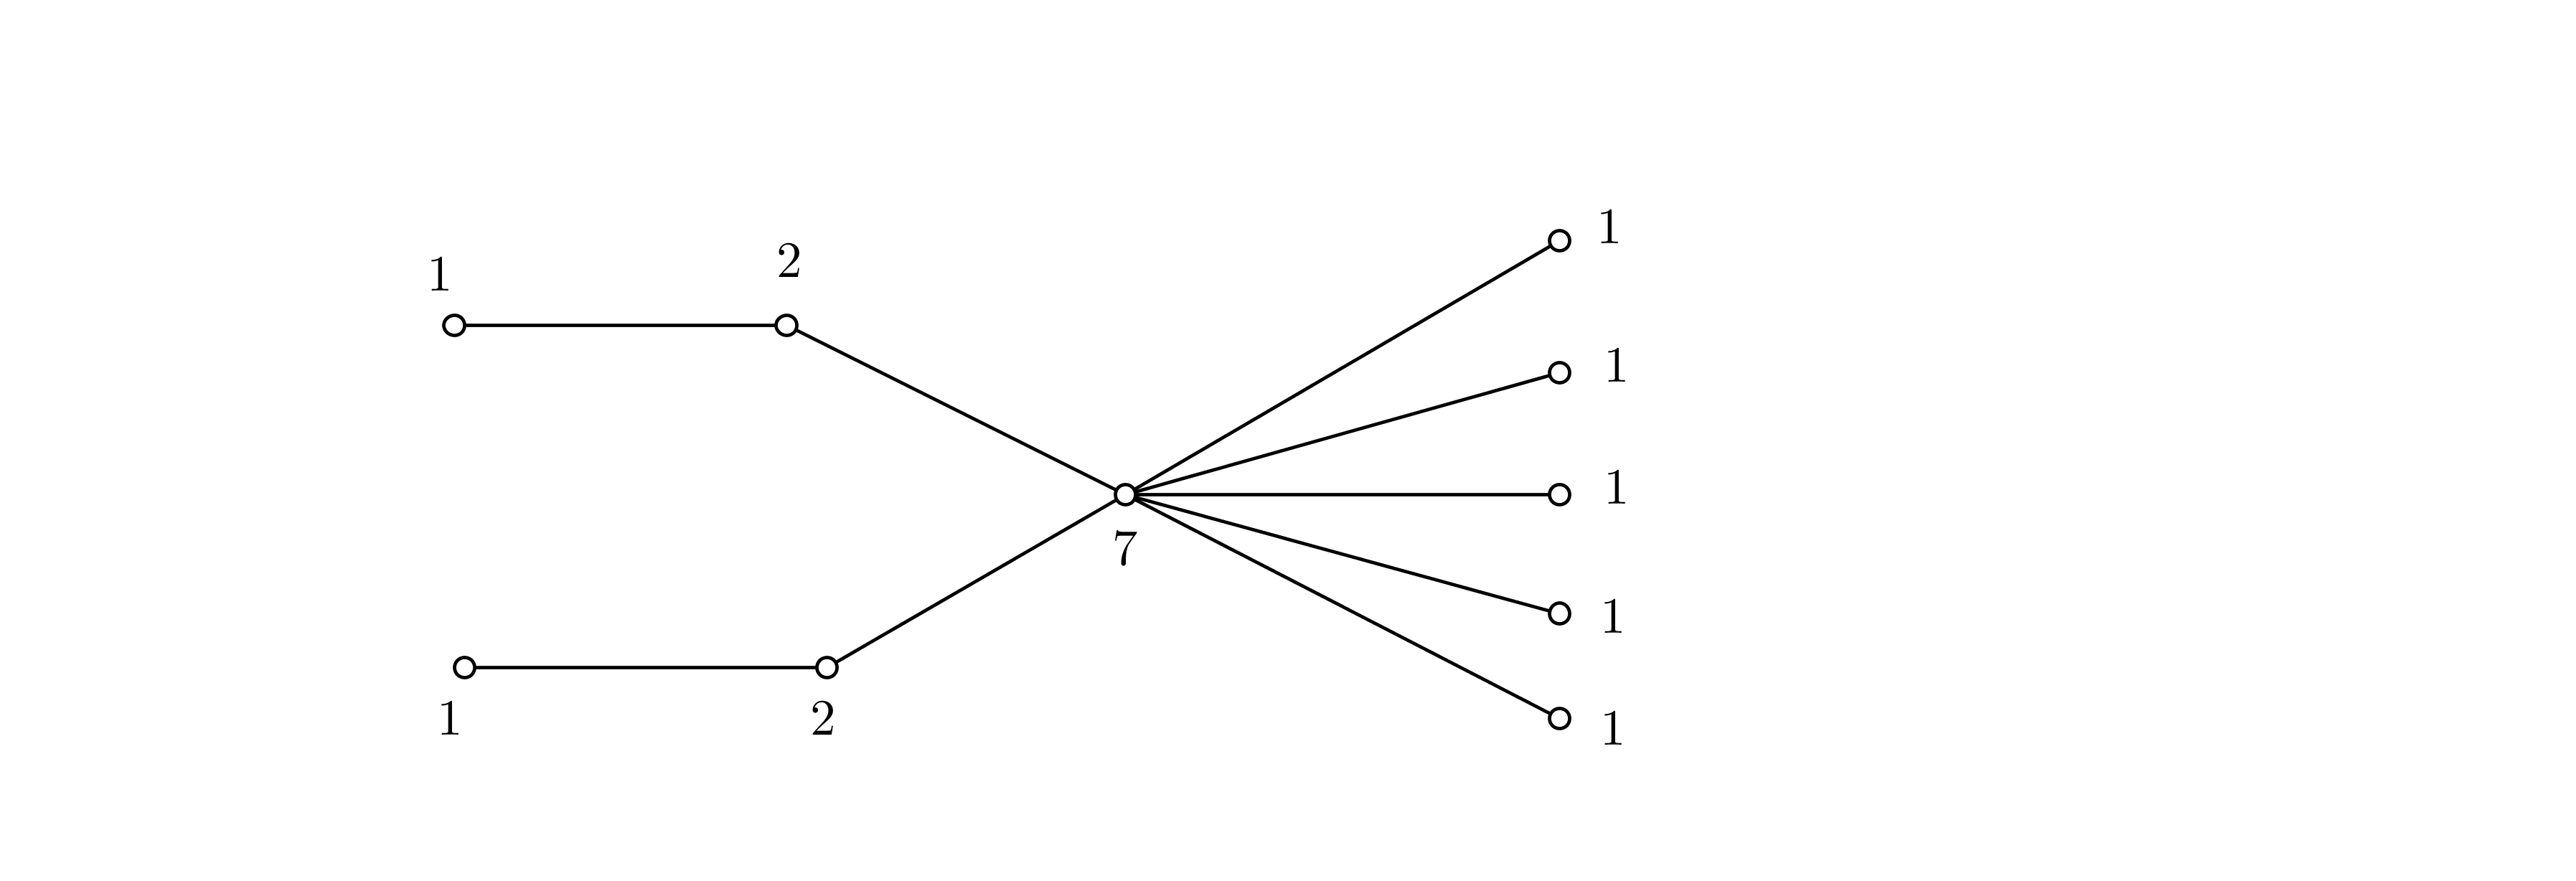
\includegraphics[width=1.0\textwidth]{SolGrapAssp5.png}
\end{figure}


  \item From Cayley's Theorem, we have $\tau(K_n)=n^{n-2}$
  \begin{align*}
  \tau(K_{10})=10^8
  \end{align*}

  \item (a) $V=\{1,2,3,\ldots,11\}$, $E=\{12,13,24,25,36,37,48,49,510,511\}$
  \begin{figure}[hbt!]
\centering
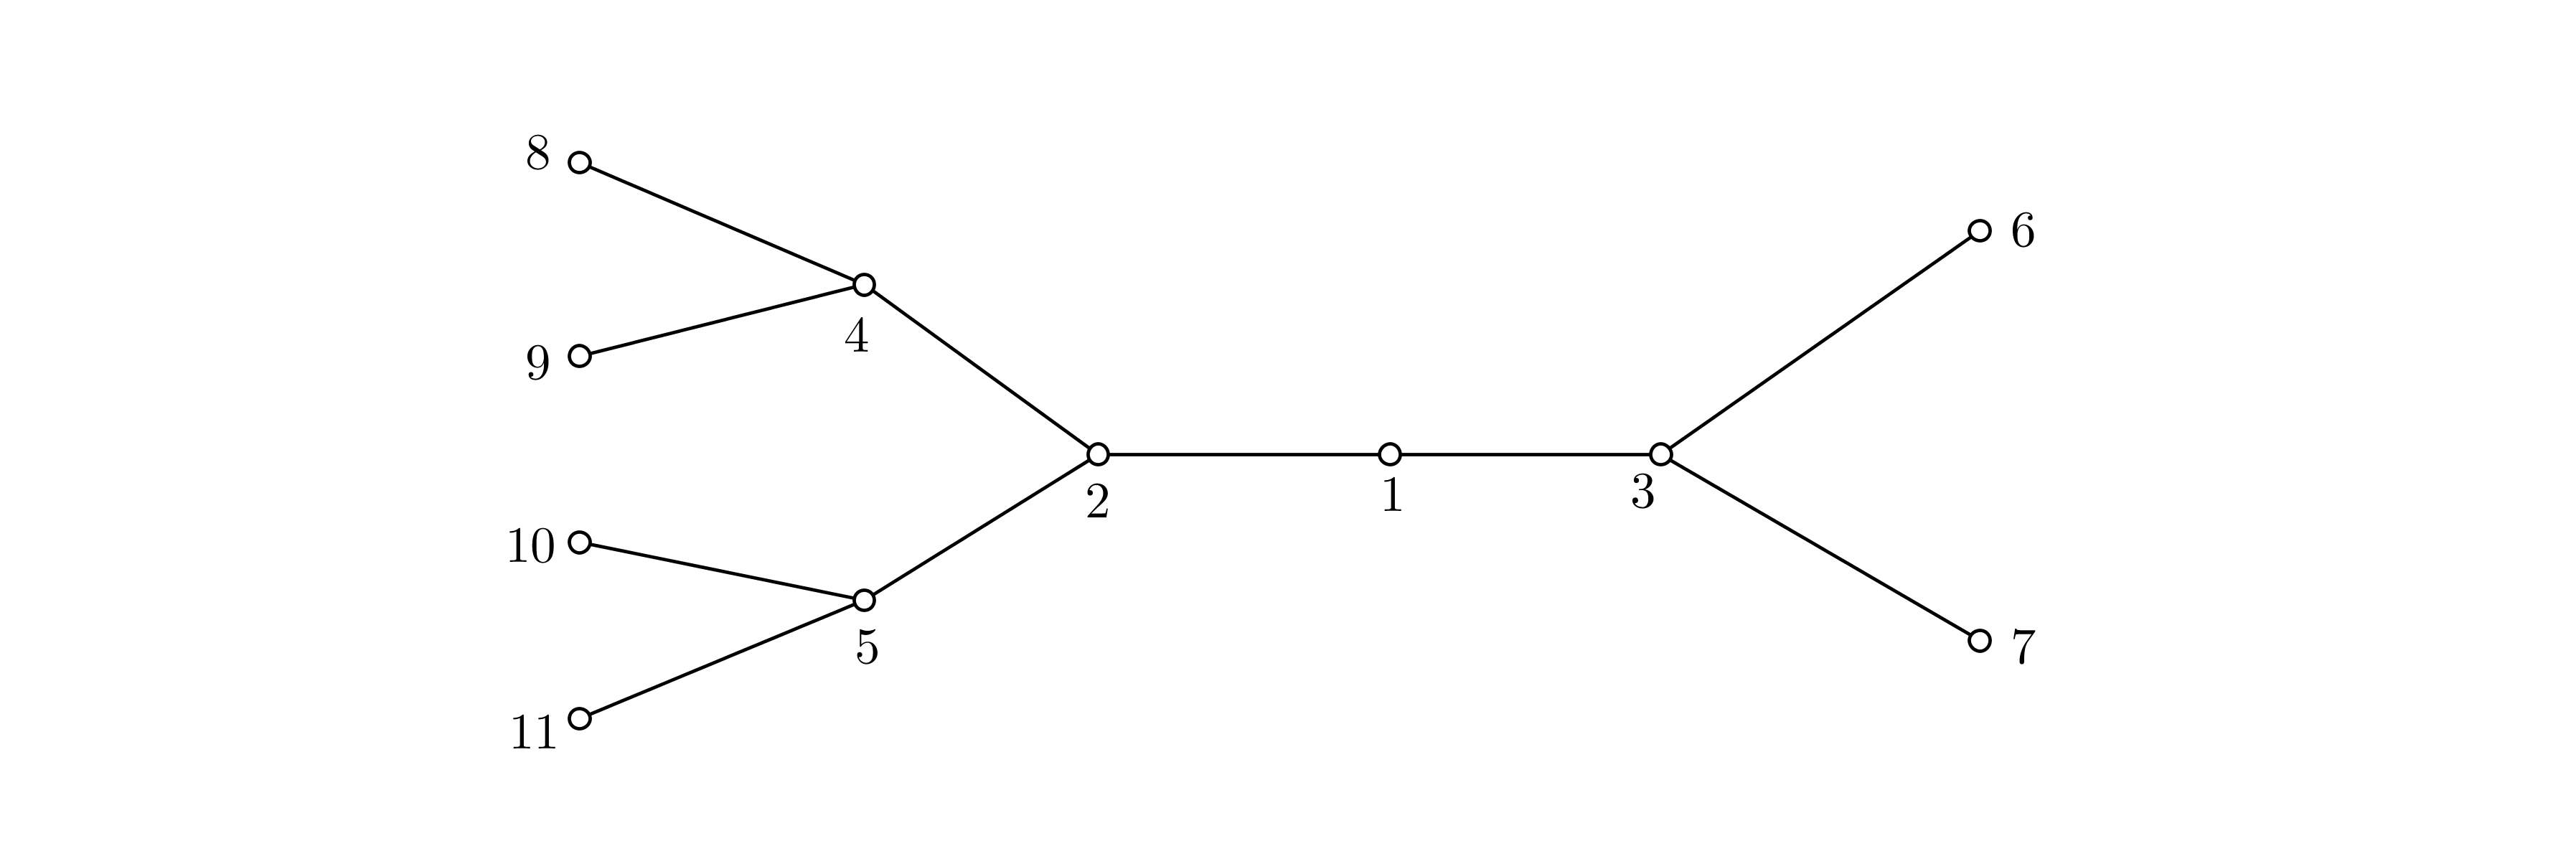
\includegraphics[width=1.0\textwidth]{SolGrapAssp7.png}
\end{figure}

  $3,3,1,2,4,4,2,5,5$ is the corresponding pr\"{u}fer sequence.\\

  (b) We have assumed $V=\{1,2,\ldots,11\}$\\
  For the pr\"{u}fer code $4,5,7,2,1,1,6,6,7$, the corresponding tree is
  \begin{figure}[hbt!]
\centering
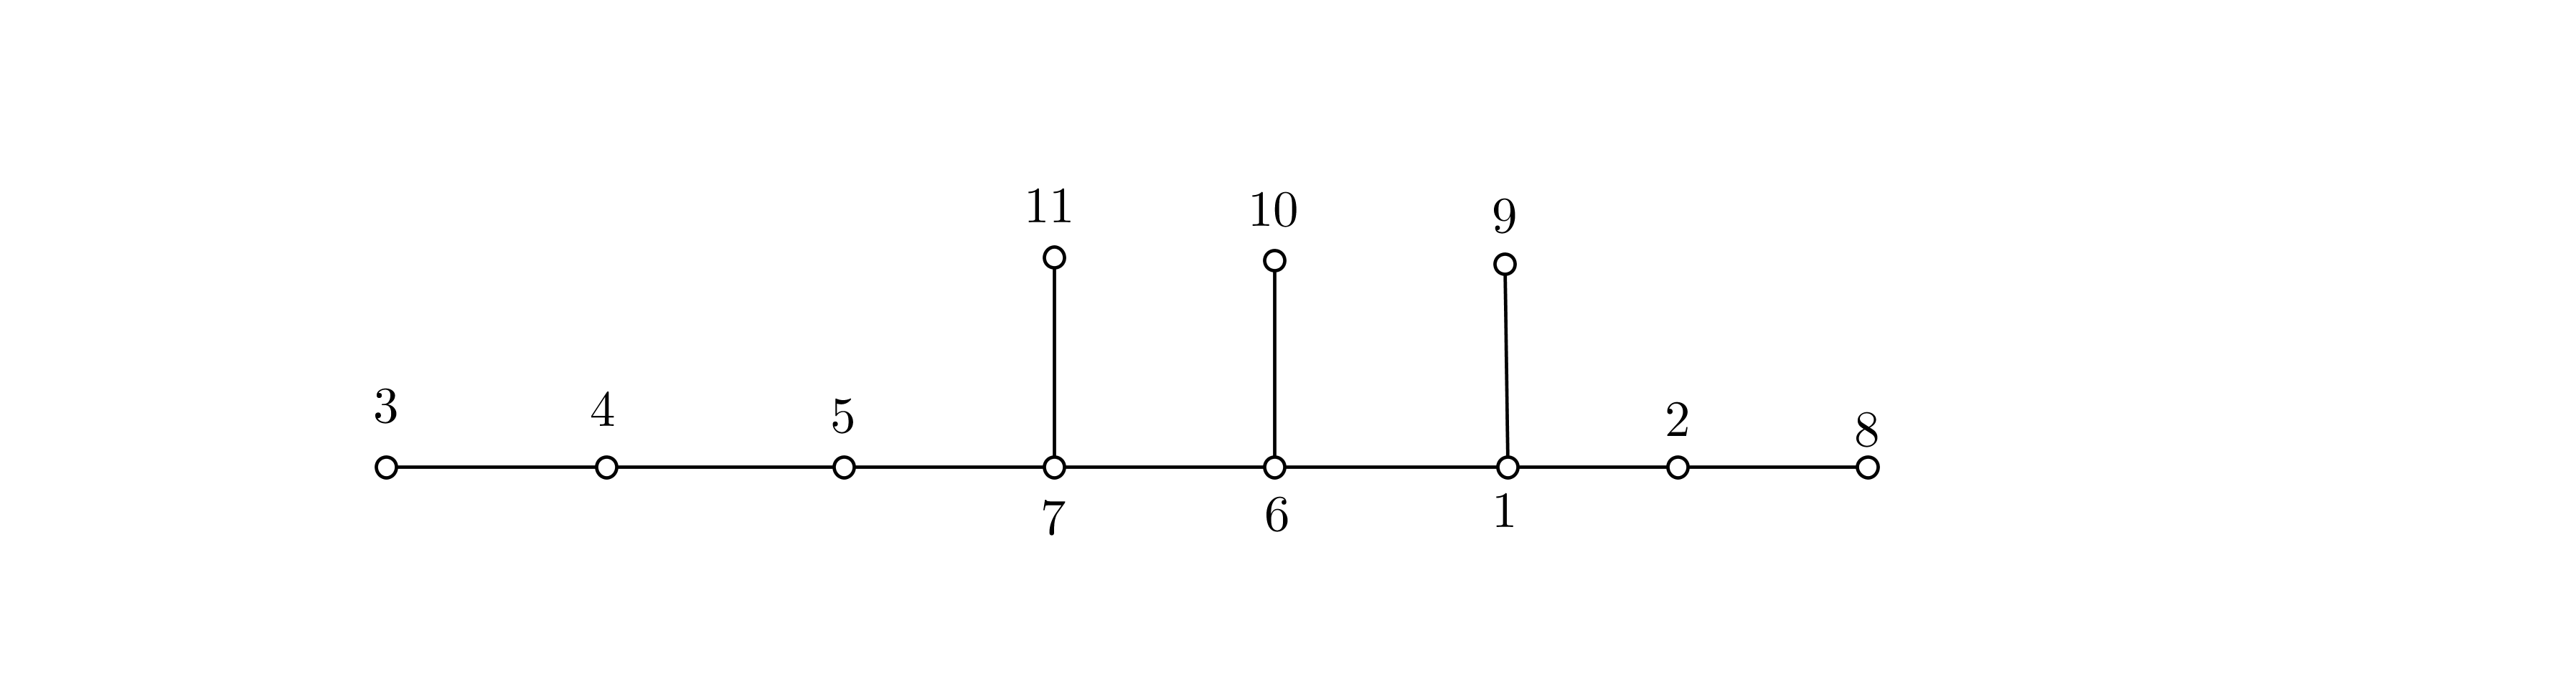
\includegraphics[width=1.0\textwidth]{SolGrapAssp7b.png}
\end{figure}

  \item $m-1$ edges.

  \item (a) There has to be two vertices of degree one in a tree of order $n\geq2$.
  (b) The maximum possible number of pendant vertices in a tree of order $n$ is $n-1$.

  \item (a) $M=\{1a,2b,3d,4c\}$
  \begin{figure}[hbt!]
\centering
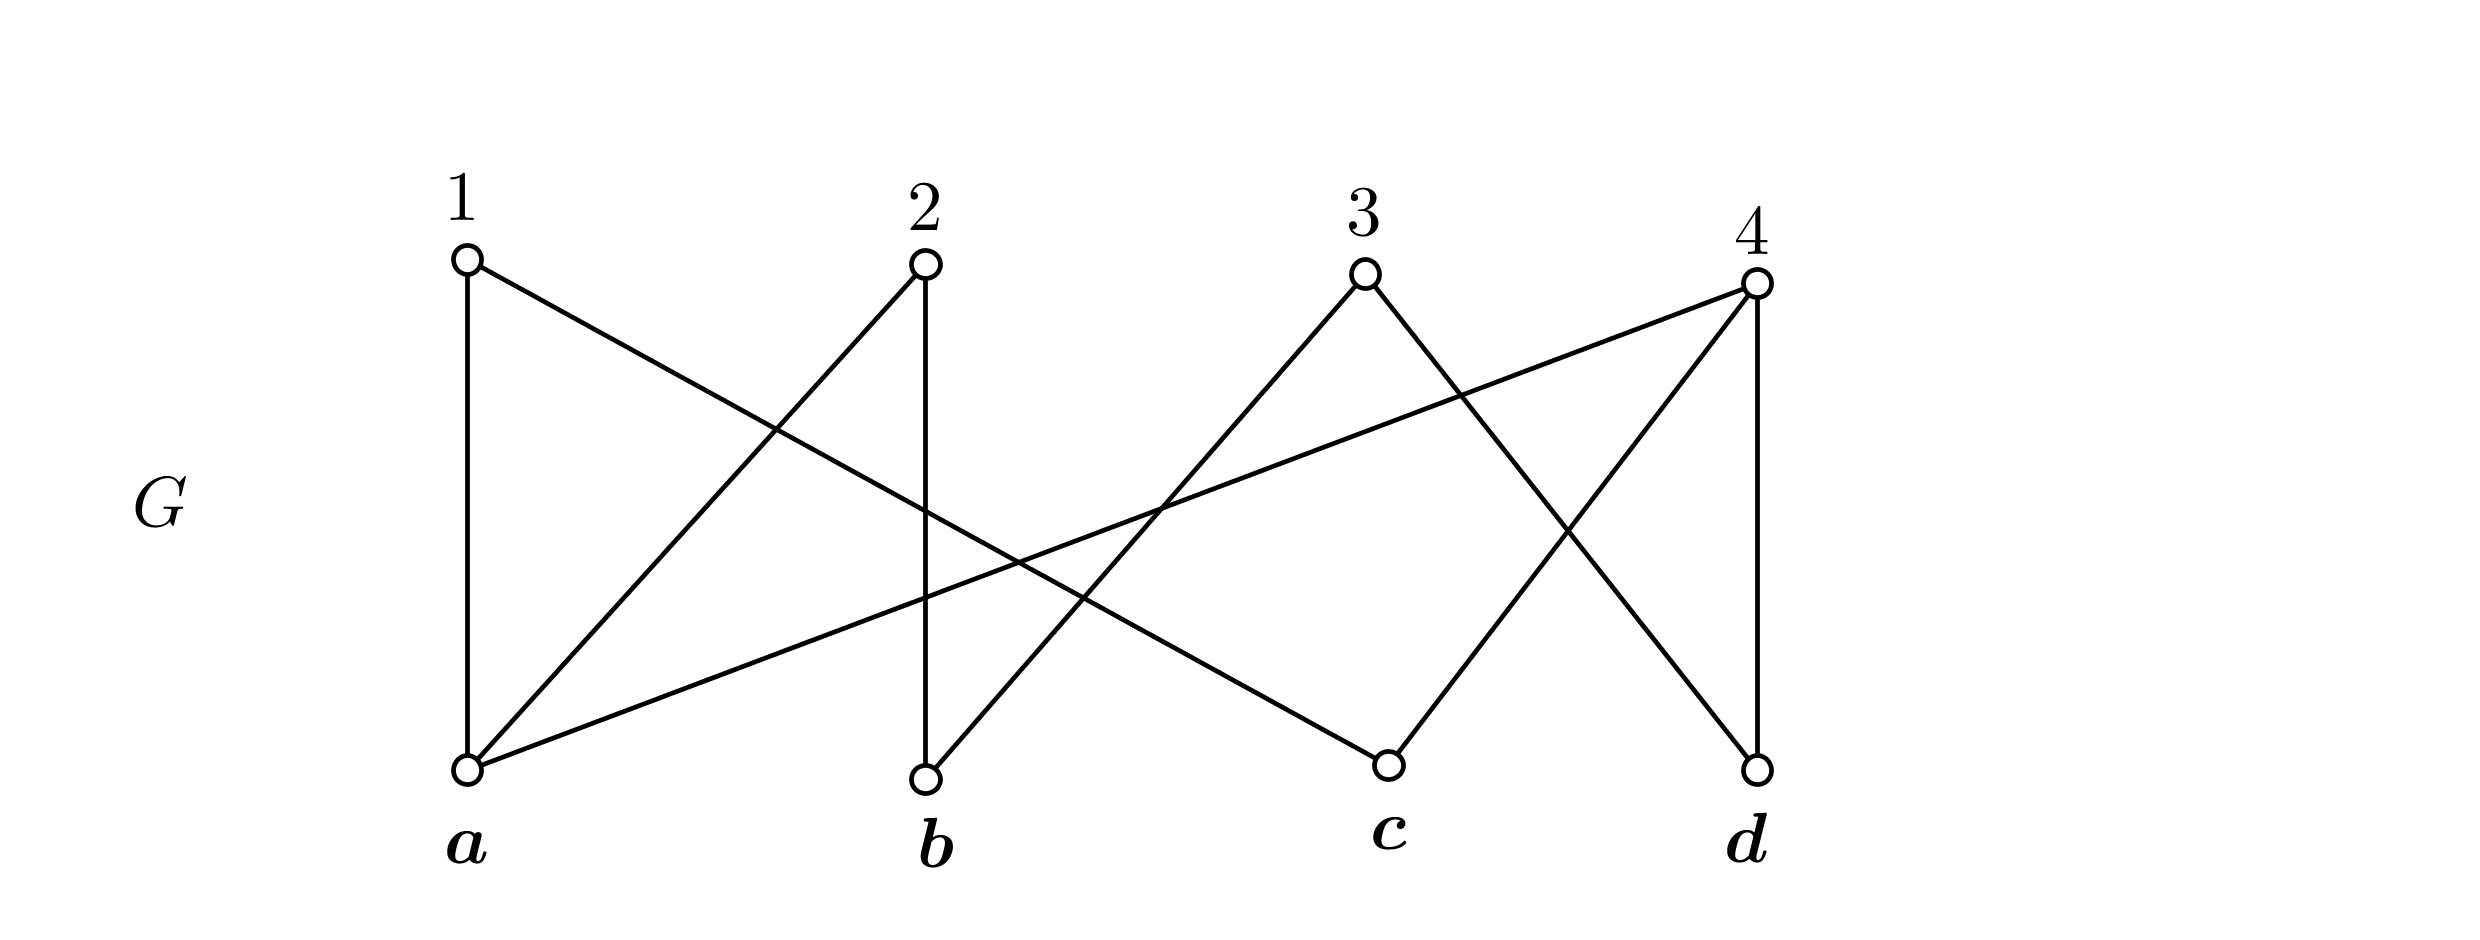
\includegraphics[width=.8\textwidth]{SolGrapAssp10a.png}
\end{figure}

  $M$ saturates $G$(i.e. $M$ is a perfect matching).\\
  (b) $M=\{Ba,Cb,Dd\}$

  \begin{figure}[hbt!]
\centering
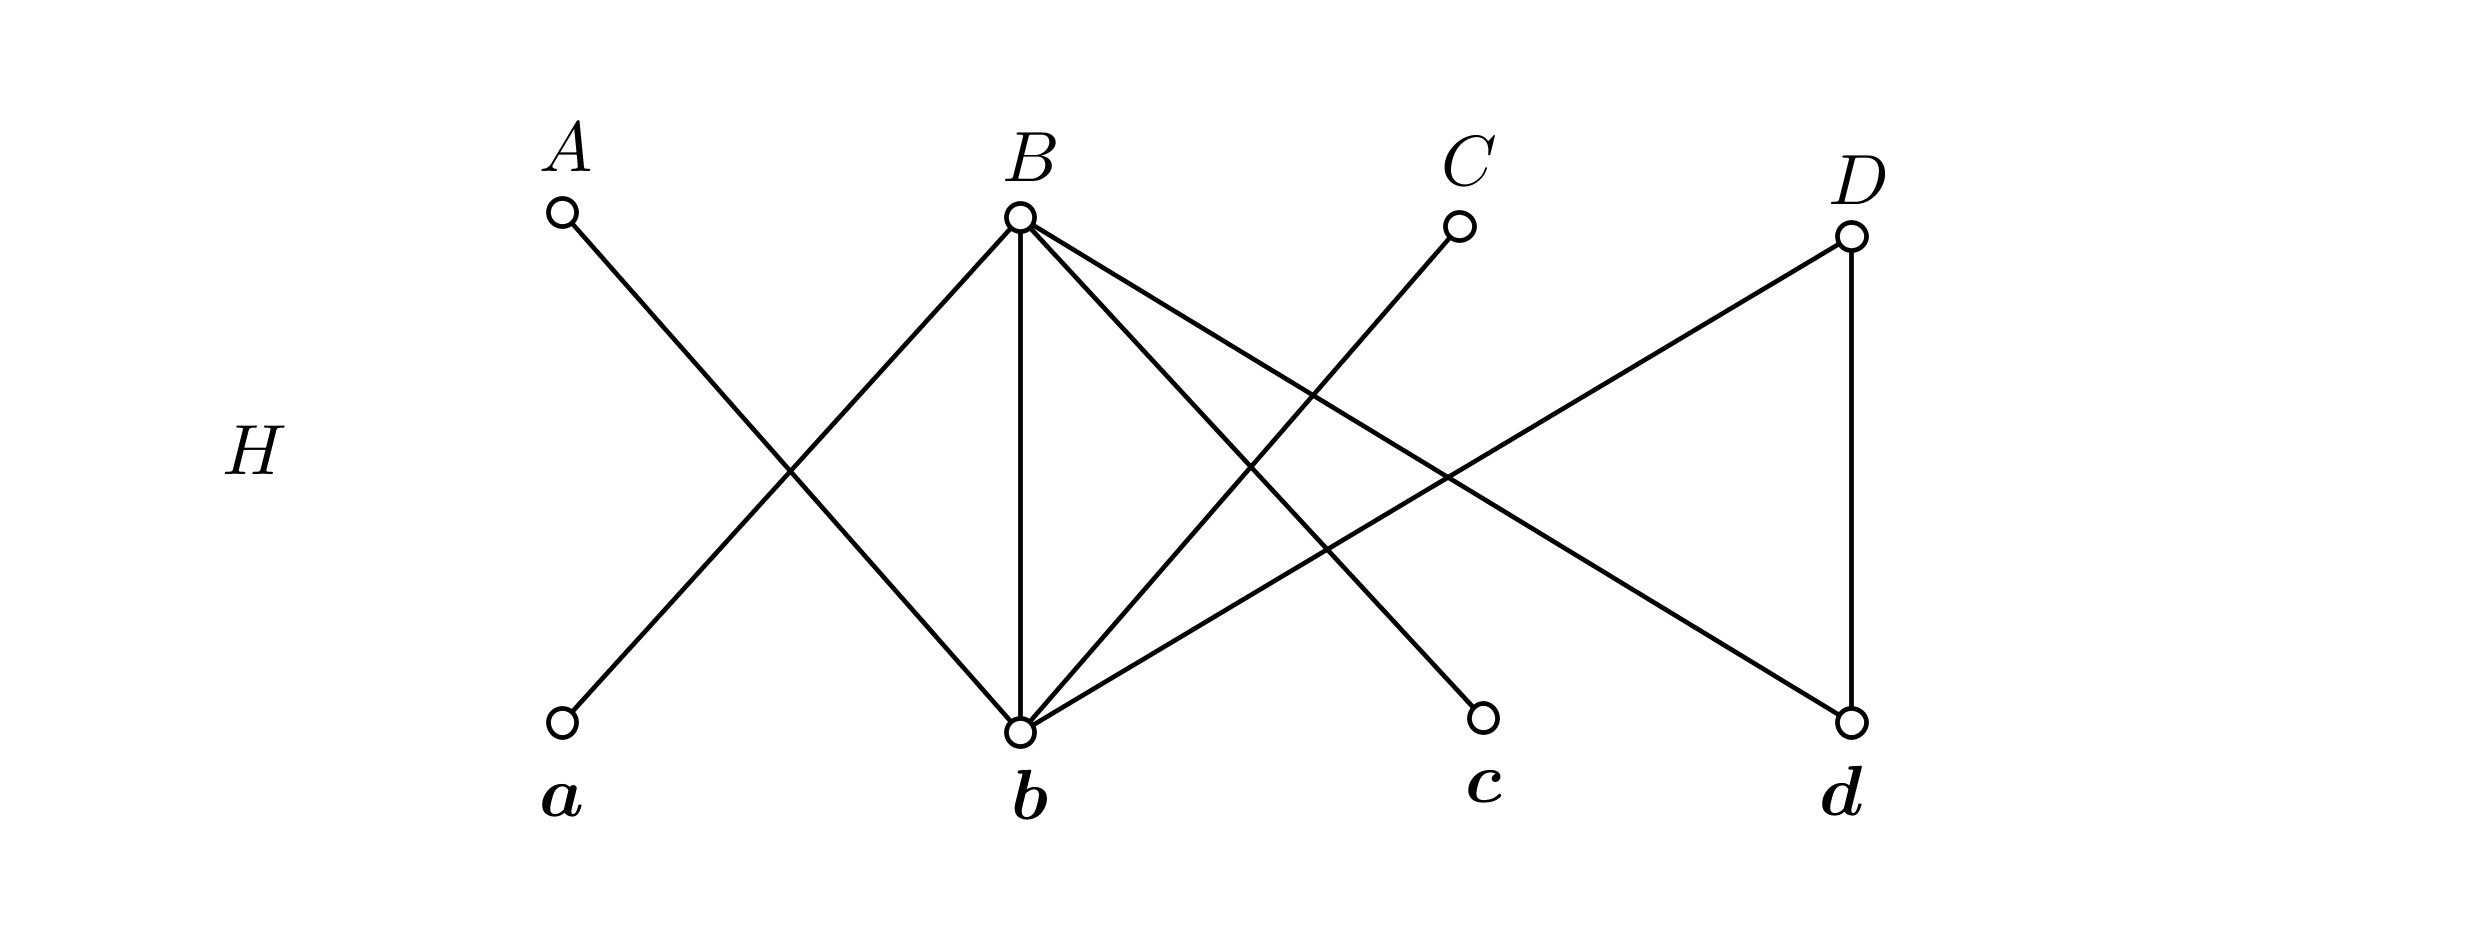
\includegraphics[width=.8\textwidth]{SolGrapAssp10b.png}
\end{figure}

  $M$ is a maximum matching. Here, there is no perfect matching because Hall's condition is not satisfied. Take $S=\{a,c,d\}$, $N(S)=\{B,D\}$
  \begin{align*}
  \Rightarrow |N(s)|=2\geq 3=|S|,\qquad \rightarrow\leftarrow
  \end{align*}

  \item It is a matter of finding a perfect matching in $G$. But Hall's Theorem tells us it is impossible to find such matching. Take $S=\{A,B,D\}$. Thus $N(S)=\{c,d\}$
      \begin{align*}
      \Rightarrow |N(S)|=2, |S|=3 \Rightarrow |N(S)|<|S|
      \end{align*}
  Therefore, there is no job for each of the applicants.
  \item Given $G$ is $4$-regular planar graph of order $n$ and $f=10$.\\
  From Euler formula we have
  \begin{align}\label{eulerformula}
  V+f-e=2
  \end{align}
  But since $G$ is $4$-regular,
  \begin{align*}
  \sum_{v\in V(G)}\deg(v)=4V=2e
  \end{align*}
  This implies
  \begin{align}\label{euresult}
  e=2V
  \end{align}
  Now, substitute (\ref{euresult}) in (\ref{eulerformula})
  \begin{align*}
  V+f-2V=2
  \end{align*}
  After simplification
  \begin{align*}
  V=f-2
  \end{align*}
  But $f=10$ is given. Hence
  \begin{align*}
  V=8
  \end{align*}
  Therefore, the order of $G$ is equal to $8$.

  \item $K_n$ is planar for $n\leq4$.
  \item For $m=1,2$ and $\forall n\in \mathbb{N}$, $K_{m,n}$ is planar.
  \item The graph in \textcolor{blue}{blue} is the dual of $G$.

  \begin{figure}[hbt!]
\centering
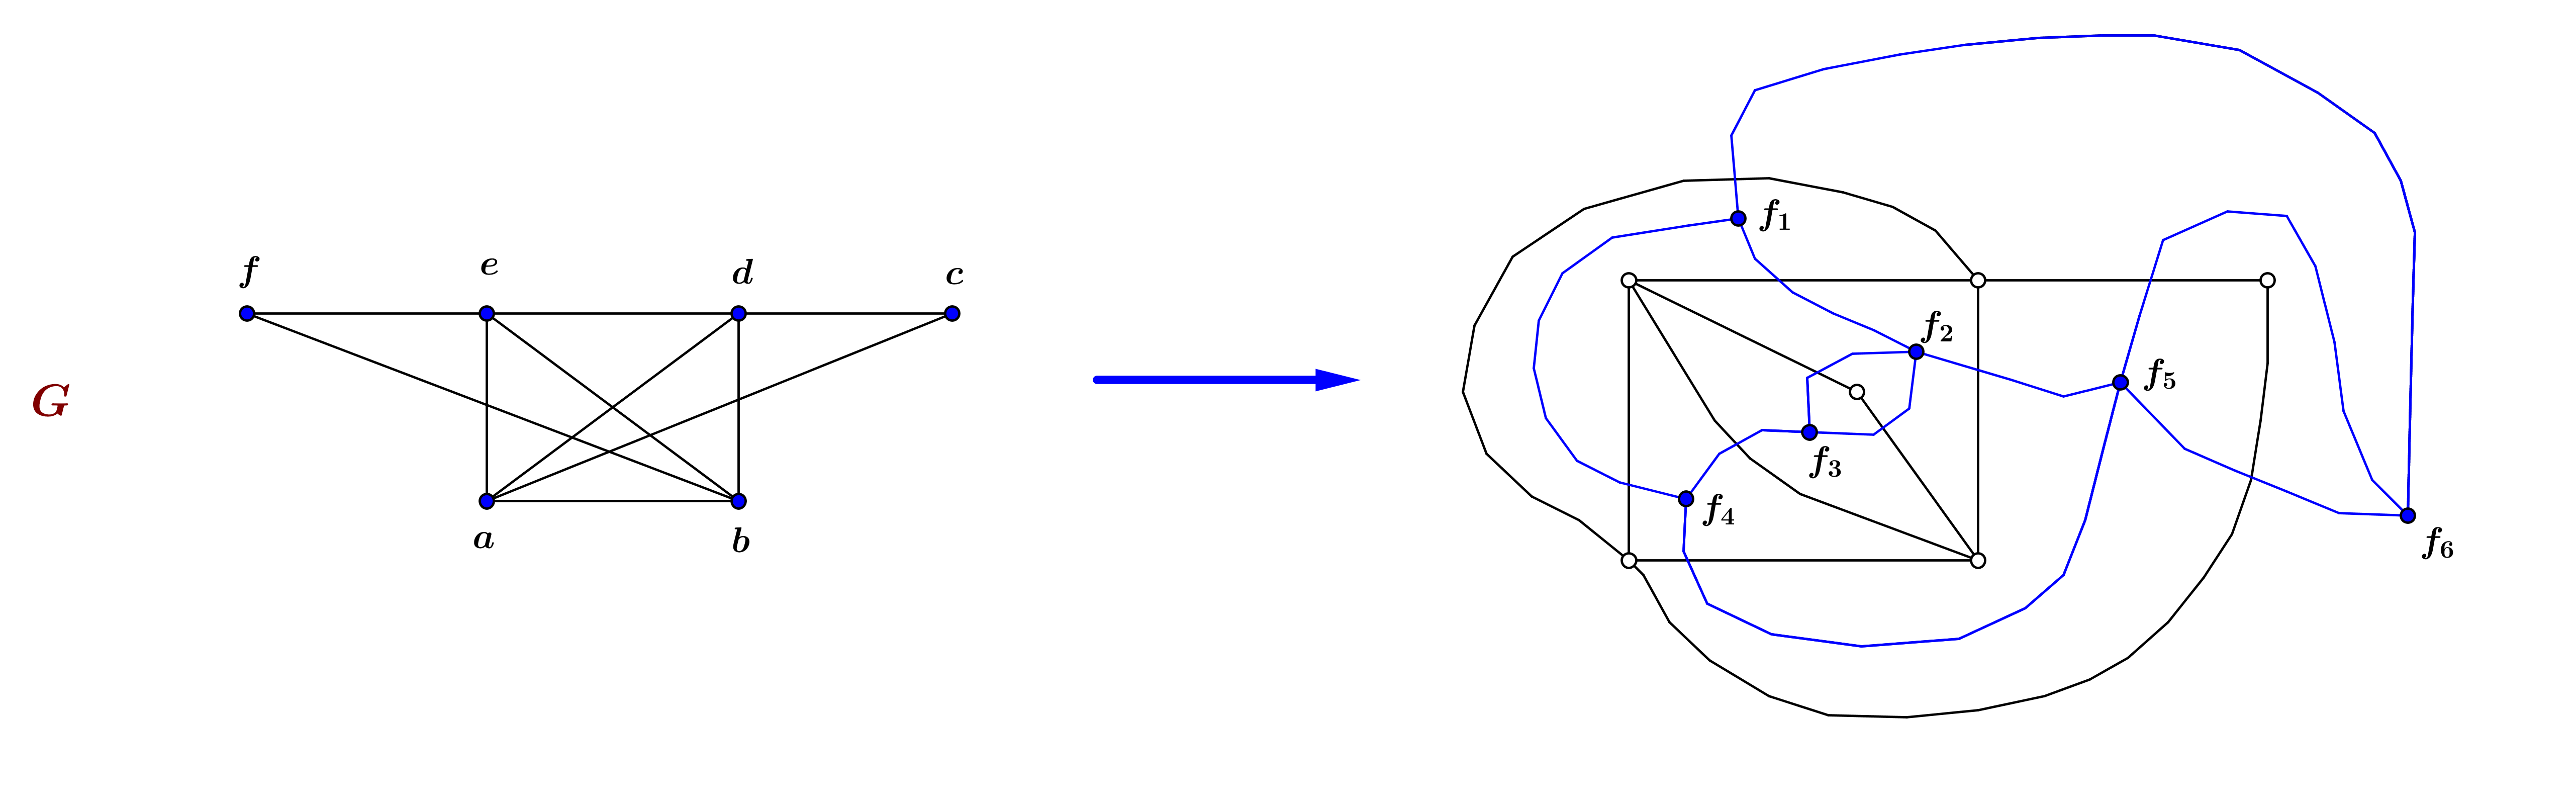
\includegraphics[width=1.0\textwidth]{Soldual.png}
\end{figure}

  The number of edges in $G$, $|E|=10$. Now
  \begin{align*}
  \sum_{i=1}^{6}\deg(f_i)&=3+4+3+3+4+3\\
                         &=20\\
                         &=2(10)=2|E|
  \end{align*}
  Therefore,
  \begin{align*}
  \sum_{\text{all faces}}\deg(\text{face})=2|E|
  \end{align*}
\end{enumerate}
\end{document}
